\documentclass[fleqn,usenatbib]{mnras}
%
%\hypersetup{draft}  %%% only for draft

%\usepackage{natbib}
\usepackage{xr-hyper}

%from mnras:
\usepackage{hyperref}	% Hyperlinks
\hypersetup{colorlinks=true,linkcolor=blue,citecolor=blue,filecolor=blue,urlcolor=blue}

\usepackage[russian]{babel}
\usepackage[utf8]{inputenc}

\usepackage{mathptmx}
\usepackage[T1]{fontenc}
\usepackage{ae,aecompl}
\usepackage{graphicx}	% Including figure files
\usepackage{amsmath}	% Advanced maths commands
\usepackage{amssymb}	% Extra maths symbols
\usepackage{multicol}   % Multi-column entries in tables
\usepackage{bm}         % Bold maths symbols, including upright Greek
\usepackage{pdflscape}  % Landscape pages
\usepackage{enumitem}
\usepackage{xspace}
\usepackage{hhline}
\def\beq#1{\begin{equation}\label{#1}}
\def\eeq{\end{equation}}

\usepackage{comment}

\usepackage{color}
\newcommand{\red}[1]{\textcolor{red}{#1}}
\newcommand{\blue}[1]{\textcolor{blue}{#1}}
\newcommand{\green}[1]{\textcolor{green}{#1}}
\newcommand{\achtung}[1]{\textcolor{red}{//#1//}}


\title[ShortTitle]{Title}
\author[Borisov et al.]{Victor Borisov, Alexander Meshcheryakov %\newauthor 
}
\date{September 2020}

%%%%%%%%%%%%%%%%%%%%
%DO NOT CHANGE
\makeatletter
\newcommand*{\addFileDependency}[1]{% argument=file name and extension
  \typeout{(#1)}
  \@addtofilelist{#1}
  \IfFileExists{#1}{}{\typeout{No file #1.}}
}
\makeatother

\newcommand*{\myexternaldocument}[1]{%
    \externaldocument{#1}%
    \addFileDependency{#1.tex}%
    \addFileDependency{#1.aux}%
}
%%%%%%%%%%%%%%%%%%%%
%CHANGE
%\myexternaldocument{pdf_figures}
%%%%%%%%%%%%%%%%%%%

\begin{document}
\maketitle
\begin{abstract}
Проведено исследование, построение и сравнение моделей вероятностных прогнозов фотометрических красных смещений (photo-z) на основе алгоритма случайного леса  с использованием данных современных астрономических обзоров SDSS, PanStarrs и DESI Legacy Survey для построения трехмерной карты квазаров.

Предложена модель photo-z, значительно превосходящая (в ~2 раза) по точности (метрики точечных прогнозов — нормализованное медианное абсолютное отклонение NMAD и доля выбросов n>0.15) лучшие модели (SOTA) известные в литературе. Для рентгеновских источников в тестовой области неба Stripe82X получена точность NMAD = 0.034 / 0.064 / 0.067 и n>0.15 = 0.079 / 0.170 / 0.163 для предложенной модели / шаблонной модели Ananna, 2017 / нейросетевой модели Brescia, 2019, соответственно.
\end{abstract}

% ===============================================================================
% ===============================================================================
% ===============================================================================


\section{Inctoduction}

On July 13, 2019 the SRG X-ray observatory
was launched from the Baikonur cosmodrome. On Dec. 8th, 2019 SRG started its first All-Sky Survey, which will consist of 8 repeated six month long scans of the entire sky. eROSITA telescope \citep{2020arXiv201003477P} onboard SRG operates in the soft X-ray band (0.3–8\,keV) and will detect $\sim3$ millions X-ray AGNs at the end of survey. In order to construct a large-scale structure map of X-ray Universe with eROSITA, accurate measurements of cosmological redshifts for extragalactic X-ray sources (mostly quasars) are needed.

Redshift measurement methods \citep{2019NatAs...3..212S} can be divided into spectroscopic (spec-z, $z_{sp}$) and photometric (photo-z, $\hat{z}_{ph}$). Spec-z's are time consuming task for faint optical objects ($r\gtrsim22^{mag}$). On the other hand, photo-z measurements can be based on data from modern large photometric sky surveys, it is much cheaper in observational resources than spec-z but also less accurate. 

In this work we present machine learning models for X-ray sources probabilistic photo-z predictions, based on photometric data from 4 modern sky surveys (SDSS, Pan-STARRS1, DESI Legacy Imaging Survey, and WISE).

% ===============================================================================
% ===============================================================================
% ===============================================================================

\section{Data}
\subsection{Photometric data}
We use photometric data from SDSS DR14 \citep{2018ApJS..235...42A}, Pan-STARRS1 DR2 \citep{2018AAS...23110201C}, DESI LIS DR8 \citep{2019AJ....157..168D} and WISE \citep{2010AJ....140.1868W} sky surveys (WISE forced photometry is taken from DESI LIS).
\subsection{Features Set}
Для построения моделей Photo-z мы строим экспертный набор признаков. Для этого сначала из потоков вычисляются величины с использованием гиперболического синуса:
\begin{equation}\label{eq:asinhmag}
    mag = \Bigg[asinh\Bigg(\frac{flux}{2 \times \sigma_{flux}}\Bigg) + \log(\sigma_{flux})\Bigg] \times \Bigg(\frac{-2.5}{\log 10}\Bigg) ~,
\end{equation}
где $flux$ и $\sigma_{flux}$ - значение и ошибка потока.

Описать свойства гиперболического синуса.

Вычисление величин по такой формуле позволяет использовать информацию об объектах с с отрицательными потоками. Кроме того вычисленные по такой формуле величины содержат в себе информацию об ошибках.

Ниже в таблицах \ref{tab:featuressets} и \ref{tab:models} описываются используемые наборы признаков и какие модели какие наборы признаков используют (криво!). 

\begin{table*}
	\begin{tabular}{ r p{10cm} }
	\hline
	    Features type & Features \\
    \hline
        SDSS mags & \(u_{SDSS,psf}\), \(g_{SDSS,psf}\), \(r_{SDSS,psf}\), \(i_{SDSS,psf}\), \(z_{SDSS,psf}\), \(u_{SDSS,cmodel}\), \(i_{SDSS,cmodel}\), \\
        SDSS colors & \(u_{SDSS,psf}-g_{SDSS,psf}\), \(u_{SDSS,psf}-r_{SDSS,psf}\), \(u_{SDSS,psf}-i_{SDSS,psf}\), \(u_{SDSS,psf}-z_{SDSS,psf}\), \(u_{SDSS,psf}-u_{SDSS,cmodel}\), \(g_{SDSS,psf}-i_{SDSS,psf}\), \(g_{SDSS,psf}-g_{SDSS,cmodel}\), \(r_{SDSS,psf}-i_{SDSS,psf}\), \(i_{SDSS,psf}-z_{SDSS,psf}\), \(i_{SDSS,psf}-i_{SDSS,cmodel}\), \\
    \hline
        Pan-STARRS mags (1) & \(g_{PS,psf}\), \(r_{PS,psf}\), \(i_{PS,psf}\), \(z_{PS,psf}\), \(y_{PS,psf}\), \(i_{PS,kron}\), \(y_{PS,kron}\) \\
        Pan-STARRS mags (2) & \(g_{PS,kron}\), \(r_{PS,kron}\), \(z_{PS,kron}\) \\
        Pan-STARRS colors (1) & \(g_{PS,psf}-i_{PS,psf}\), \(g_{PS,psf}-y_{PS,psf}\), \(r_{PS,psf}-i_{PS,psf}\), \(r_{PS,psf}-y_{PS,psf}\), \(i_{PS,psf}-z_{PS,psf}\), \(i_{PS,psf}-y_{PS,psf}\), \(z_{PS,psf}-y_{PS,psf}\), \(i_{PS,psf}-i_{PS,kron}\), \(y_{PS,psf}-y_{PS,kron}\) \\
        Pan-STARRS colors (2) & \(g_{PS,psf}-r_{PS,psf}\) \(g_{PS,psf}-z_{PS,psf}\), \(r_{PS,psf}-z_{PS,psf}\), \(g_{PS,psf}-g_{PS,kron}\), \(r_{PS,psf}-r_{PS,kron}\), \(z_{PS,psf}-z_{PS,kron}\) \\
    \hline
        DESI LIS mags & \(g_{LS}\), \(r_{LS}\), \(z_{LS}\) \\
        DESI LIS colors & \(g_{LS}-r_{LS}\), \(g_{LS}-z_{LS}\), \(r_{LS}-z_{LS}\) \\
    \hline
        WISE mags & \(w1\), \(w2\) \\
        WISE colors & \(w1-w2\) \\
    \hline
        SDSS + DESI LIS colors & \(g_{SDSS,cmodel}-g_{LS}\), \(r_{SDSS,cmodel}-r_{LS}\), \(z_{SDSS,cmodel}-z_{LS}\) \\
        SDSS + WISE colors & \(u_{SDSS,cmodel}-w1\), \(u_{SDSS,cmodel}-w2\), \(g_{SDSS,cmodel}-w1\), \(g_{SDSS,cmodel}-w2\), \(r_{SDSS,cmodel}-w1\), \(r_{SDSS,cmodel}-w2\), \(i_{SDSS,cmodel}-w1\), \(i_{SDSS,cmodel}-w2\), \(z_{SDSS,cmodel}-w1\), \(z_{SDSS,cmodel}-w2\) \\
        Pan-STARRS + DESI LIS colors & \(g_{PS,kron}-g_{LS}\), \(r_{PS,kron}-r_{LS}\), \(z_{PS,kron}-z_{LS}\) \\
        Pan-STARRS + WISE colors & \(g_{PS,kron}-w1\), \(g_{PS,kron}-w2\), \(r_{PS,kron}-w1\), \(r_{PS,kron}-w2\), \(i_{PS,kron}-w1\), \(i_{PS,kron}-w2\), \(z_{PS,kron}-w1\), \(z_{PS,kron}-w2\), \(y_{PS,kron}-w1\), \(y_{PS,kron}-w2\) \\
        DESI LIS + WISE & \(g_{LS}-w1\), \(g_{LS}-w2\), \(r_{LS}-w1\), \(r_{LS}-w2\), \(z_{LS}-w1\), \(z_{LS}-w2\) \\
    \hline
    \end{tabular}
    \label{tab:featuressets}
    \caption{Описание наборов используемых признаков (величины, вычисленные по формуле гиперболического синуса \eqref{eq:asinhmag} и цвета на основе этих величин).}
\end{table*}

\begin{table*}[ht]
    \centering
    \begin{tabular}{r p{10cm}}
    \hline
        Model & Feature sets used \\
    \hline
        Pan-STARRS + WISE & Pan-STARRS mags (1 and 2) and colors (1 and 2), WISE mags and colors, Pan-STARRS + WISE colors \\
        DESI LIS + WISE & DESI LIS mags and colors, WISE mags and colors, DESI LIS + WISE colors \\
        Pan-STARRS + DESI LIS + WISE & Pan-STARRS mags (1) and colors (1), DESI LIS mags and colors, WISE mags and colors, Pan-STARRS + DESI LIS colors, Pan-STARRS + WISE colors \\
        SDSS + Pan-STARRS + DESI LIS + WISE & SDSS mags and colors, Pan-STARRS mags (1) and colors (1), DESI LIS mags and colors, WISE mags and colors, SDSS + WISE colors, SDSS + DESI LIS colors, Pan-STARRS + WISE colors \\
    \hline
    \end{tabular}
    \caption{Caption}
    \label{tab:models}
\end{table*}


\subsection{Account for extinction}

Для учета межзвездного поглощения используется оценки $E(B-V)$ из каталога DESI LIS и коэфициенты $A/E(B-V)$ из работы \citep{2011ApJ...737..103S}. Скорректированные значения потоков и ошибок на потоки вычисляются по следующим формулам:
\begin{equation}
    flux_{ebv, pb} = flux_{pb} 10^{0.4 * dm_{pb}},
\end{equation}
\begin{equation}
    \sigma_{flux_{ebv, pb}} = \sigma_{flux_{pb}} 10^{0.4 * dm_{pb}},
\end{equation}
где $dm_{pb} = E(B-V) * [A/E(B-V)]_{pb}$, $[A/E(B-V)]_{pb}$ -- коэфициент из \citep{2011ApJ...737..103S} для фильтра $pb$, $flux_{ebv, pb}$ и $\sigma_{flux_{ebv, pb}}$ -- значение потока и ошибка на поток в фильтре $pb$.

\subsection{Train sample}
\subsection{Stripe82X test sample}
\subsection{Test sample of DR16q objects}
\begin{table*}
	\begin{tabular}{llll}
            \hline
            {} & Train sample & Stripe82X & DR16q test \\
            \hline
            Total              &       586176 &      6195 &      58682 \\
            Number of galaxies &       136428 &       701 &          0 \\
            Number of QSO      &       449748 &      1875 &      58682 \\
            \hline
            Has DESI LIS       &      99.03\% &   92.62\% &    99.60\% \\
            Has Pan-STARRS     &      98.91\% &   71.12\% &    85.38\% \\
            Has SDSS           &      98.68\% &   74.96\% &    99.46\% \\
            \hline
            \end{tabular}
            \caption{Описание используемых выборок (количество объектов по классам (галактики, квазары) и доли объектов, имеющих фотометрию в используемых широких обзорах неба). Поскольку кросс-отождествление сначала производится с каталогом DESI LIS, а потом для компаньонов DESI LIS ищутся данные Pan-STARRS и SDSS, доли объектов с фотометрией Pan-STARRS и SDSS не больше, чем с DESI LIS.}
\end{table*}

\begin{figure*}
    \centering
    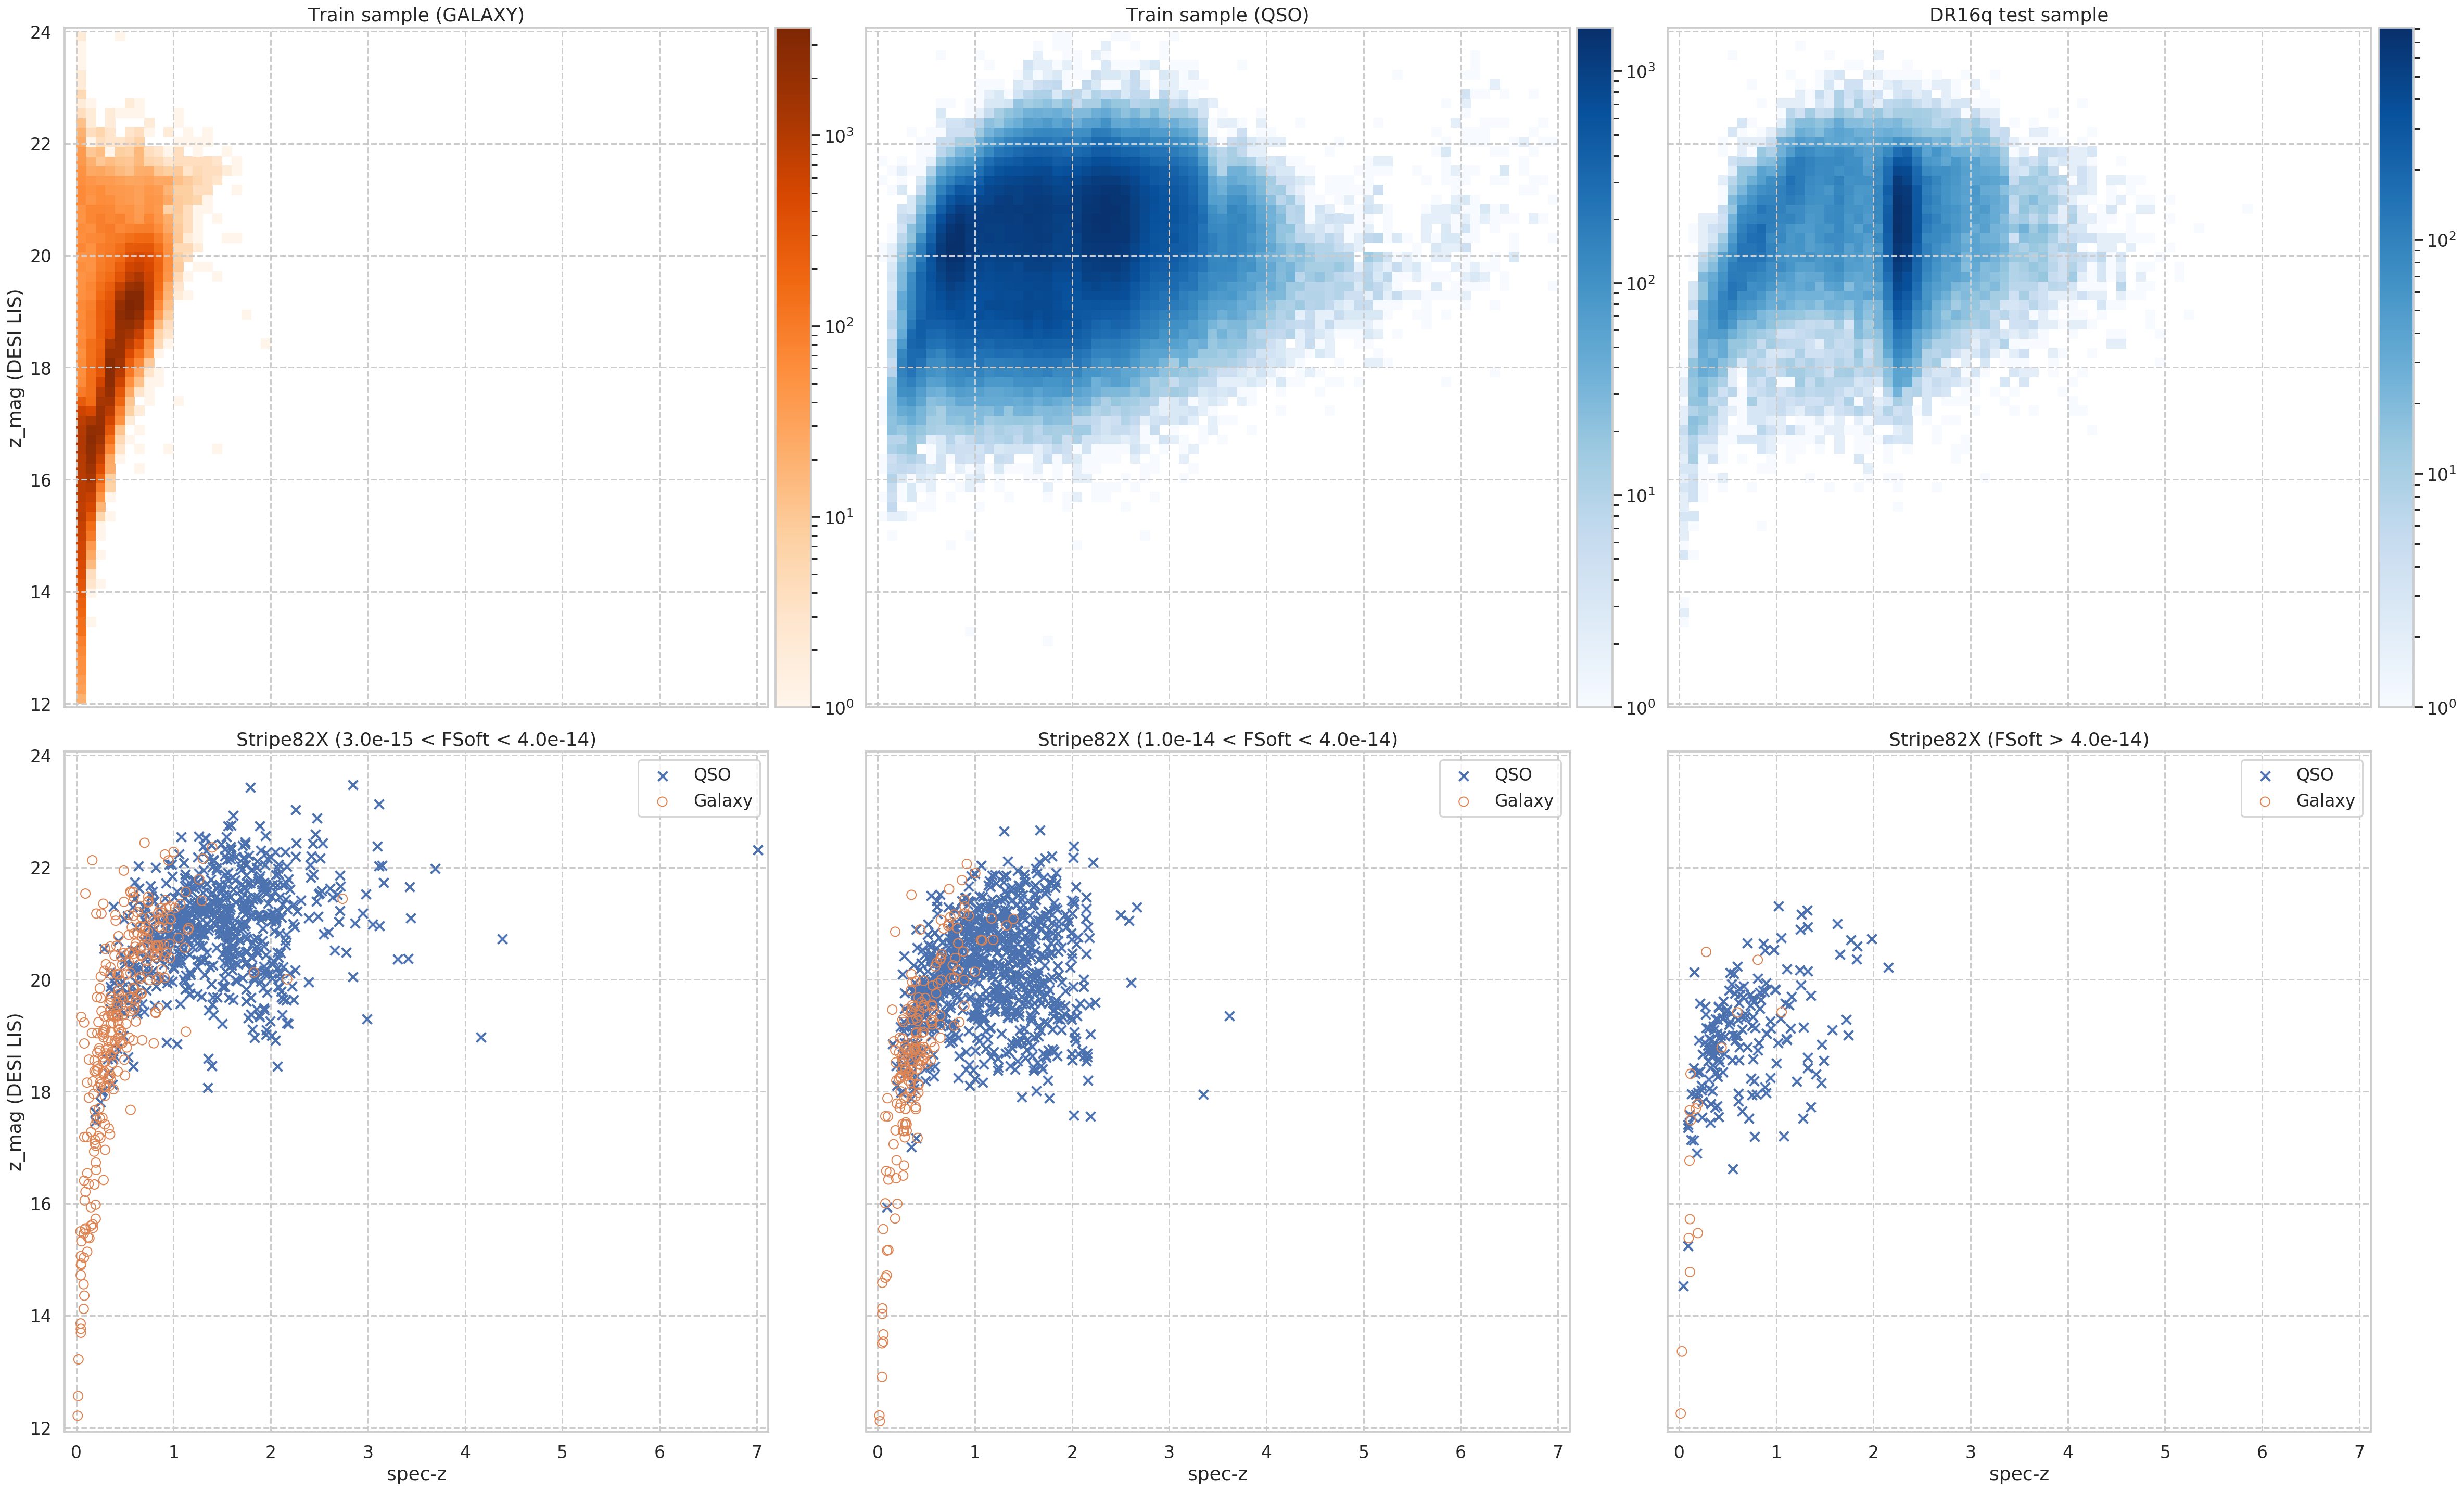
\includegraphics[width=0.95\linewidth]{images/data-dist.png}
    \caption{Распределения объектов в используемых выборках. Слева сверху -- объекты Stripe82X, оранжевыми крестиками показаны галактики, синими плюсиками -- квазары. Справа сверху -- двумерная гистограмма распределения объектов тестовой выборки квазаров SDSS DR16q. Снизу -- двумерные гисторгаммы распределения галактик (слева) и квазаров (справа) тренировочной выборки.}
    \label{fig:data_distribution}
\end{figure*}

% ===============================================================================
% ===============================================================================
% ===============================================================================

\section{The algorithm}
\subsection{Random forest}

Случайный лес \cite{bib:forests_brieman} представляет собой ансамбль деревьев, основанных на одном и том же базовом алгоритме построения дерева решений, которые строятся на случайных подвыборках одной тренировочной выборки. Каждое дерево \(A^j\) задает разбиение признакового пространства \(X\) на не пересекающиеся прямоугольные подпространства \(A^j_i\), соответствующие листьям дерева, то есть
\begin{equation}
    X = \bigcup_i {A^j_i}; A^j_n \cap A^j_m = \emptyset, n \neq m.
\end{equation}
При этом каждое дерево содержит в себе некоторую случайность построения, которая контролируется вектором гиперпараметров случайного леса \(\Theta\). Например, \(\Theta\) может задавать, по какому признаку и по какому диапазону его значений будет разбиваться очередной узел. Очень важным, что будет показано ниже, является параметр, контролирующий разбиение обучающей выборки на случайные подвыборки для построения деревьев. Таким образом, деревья, входящие в случайный лес получаются разными. Для получения финального прогноза прогнозы всех деревьев усредняются, т.е., обозначив случайный лес как ансамбль деревьев \(\mathbb{V}_T = \{A^j, 1 \leq j \leq T\}\), можно записать в виде формулы
\begin{equation}
    \hat{\eta}_{n, \mathbb{V}_T}(x) = \frac{1}{T} \sum_{j=1}^T \hat\eta_{n, A^j}(x),
\end{equation}
где \(\hat\eta_{n, A^j}(x)\) - прогноз дерева \(A^j\).

Впервые для задачи вероятностной регрессии был использован в работе Meinshausen, 2006 \cite{bib:forests_meinshausen} для точечной оценки квантилей. Построение модели заключается в обучении случайного леса с квантильной функцией потерь 
\begin{equation}
    l(y_i, \hat{y}_{\alpha, i}) = (1-\alpha)|y_i - \hat{y}_{\alpha, i}|\mathbb{I}[y \leq \hat{y}_{\alpha, i}] + \alpha|y_i - \hat{y}_{\alpha, i}|\mathbb{I}[y > \hat{y}_{\alpha, i}],
\end{equation}
где \(y_i\) - истинное значение, \(\hat{y}_{\alpha, i}\) - предсказанное значений целевой переменной.

Для задачи прогноза photo-z впервые был применен в работе \cite{bib:tpz}, где вероятностный прогноз строится как набор вероятностей того, что целевой признак заданного объекта принадлежит тому или иному интервалу значений. В работе \cite{bib:mesch} вероятностный прогноз представляет собой непрерывную функцию плотности вероятности, полученную применением ядерной оценки плотности к ансамблю прогнозов деревьев. Важно заметить, что в обоих алгоритмах используются леса, без ограничения глубины, т.е. когда в каждом листе каждого дерева находится один и только один элемент тренировочной выборки. Более подробный обзор этих алгоритмов приведен ранее в \ref{sec:phz_packages_comparison} и \ref{subsec:mesch} соответственно, где установлено, что эти алгоритмы дают лучшую точность в задаче прогноза photo-z, поэтому решено для построения моделей photo-z использовать случайный лес без ограничения глубины.

\subsection{Random forest adoptation for probabilistic predictions}
Our aim was to estimate conditional redshift distribution $p(z|x)$ for each target object with photometric features $x$.
We use Random Forest (RF) model, \citep{2001MachL..45....5B,JMLR:v7:meinshausen06a}, which is considered by many authors among the most accurate ML algorithms for photo-z measurements of galaxies \citep{2020MNRAS.499.1587S,2020arXiv200912112E} and X-ray quasars \citep{2018AstL...44..735M}. We used RF ensemble predictions in combination with gaussian Kernel Density Estimation (gKDE), to obtain $p(z|x)$. RF+gKDE model allows one to calculate photo-z point estimate $\hat{z}_{ph} = \arg\max_z p(z|x)$, confidence intervals, and $zConf = \int_{\delta z_{norm} < 0.06} p(z|x)~dz$.

At the prediction stage we take into account uncertainties in photometric fluxes of the target object, by perturbing  fluxes (according to given uncertainties) for each regression tree in the forest. Схема используемаого метода представлена на рисунке \ref{fig:qrf_scheme}.

\begin{figure}
    \centering
    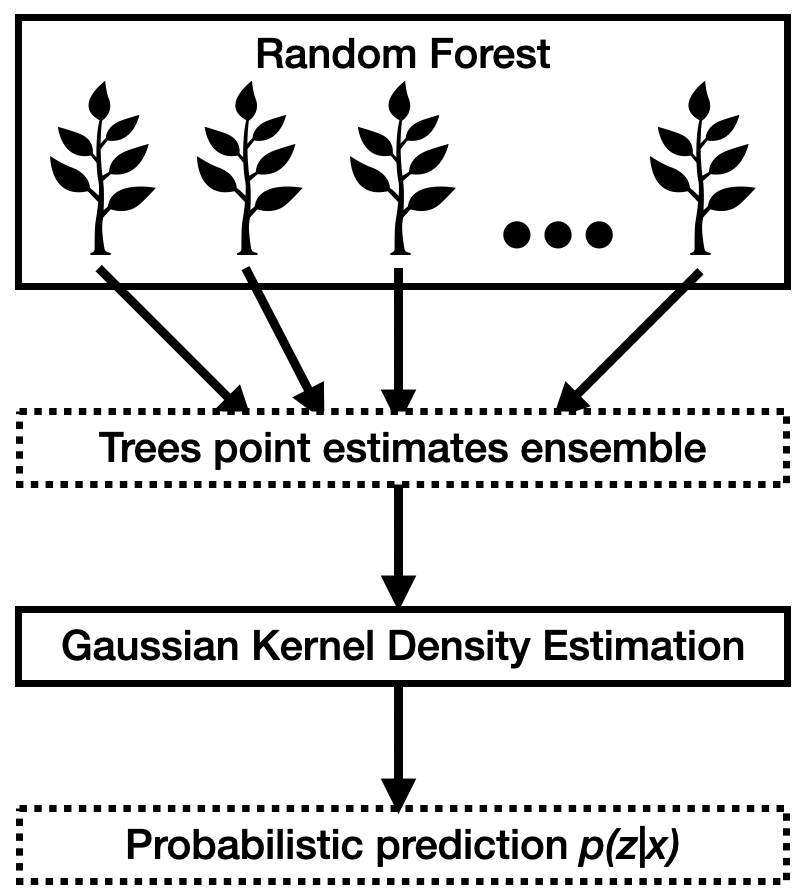
\includegraphics[width=0.95\linewidth]{images/qrf.png}
    \caption{Схема используемого алгоритма случайного леса, адоптированного для получения вероятностных прогнозов photo-z.}
    \label{fig:qrf_scheme}
\end{figure}

\section{Metrics}

В данном разделе описываются метрики качества прогнозов. В разделе \ref{sec:point-metrics} описаны метрики точечных прогнозов, разделе \ref{sec:ci-metrics} -- метрики доверительных интервалов, в \ref{sec:dist-metrics} -- метрики качества полных вероятностных прогнозов.

\subsection{Point-estimates metrics}\label{sec:point-metrics}

Чтобы оценить качество точечных прогнозов photo-z, полученных из вероятностного прогноза, мы используем 2 метрики стандартные для задачи прогнозов photo-z:
\begin{itemize}
    \item Оценка колокола распределения ошибок \begin{equation}\label{eq:nmad}
        NMAD = 1.4826 \times median(|\delta z_{norm,i}|)
    \end{equation}
    \item и долю катастрофических выбросов \begin{equation}\label{eq:n015}
        n_{>0.15} = \frac{\#\{i = \overline{1, N} | \delta z_{norm, i} > 0.15\}}{N};
    \end{equation}
\end{itemize}
где \(N\) - размер выборки, и ошибка прогноза \begin{equation}\label{eq:dznorm}
    \delta z_{norm,i} = \frac{\Delta z_i}{1+z_{spec,i}} = \frac{\hat{z}_{ph,i} - z_{spec,i}}{1+z_{spec,i}}.
\end{equation}

\subsection{Confidence intervals metrics}\label{sec:ci-metrics}

Для оценки качества калибровки доверительных интервалов мы будем сравнивать теоретический и фактический уровень доверия 68-процентных доверительных интервалов, то есть \begin{equation}\label{eq:c68}
    C_{68} - 0.68 = \frac{\#\{i = \overline{1, N} | z_{ph,i} \in CI_{68, i}\}}{N} - 0.68.
\end{equation}

\subsection{Distribution metrics}\label{sec:dist-metrics}

В качестве метрики распределений будет использоваться калибровка меры достоверности прогноза \(zConf\) \eqref{}, которая имеет смысл вероятности. Для неё будет оцениваться кумулятивная функция распределения \begin{equation}\label{eq:zconf_cal}
    F(x) = \frac{\#\{i = \overline{1, N} | zConf_i < x \}}{N}.
\end{equation}
При хорошей калибровке мы рассчитываем увидеть функцию равномерного распределения на интервале $[0, 1]$. Контролировать калибровку меры уверенности прогноза $zConf$ очень важно, поскольку она используется для отбора кандидатов в наиболее далекие квазары.

% ===============================================================================
% ===============================================================================
% ===============================================================================

\section{Results}
Нашей целью является исследование поведения моделей, построенных на разных наборах признаков (прдробнее см. в \ref{}), в зависимости от наблюдаемых предикторов (величины в фильтрах r, z, рентгеновский поток) и от целевой величины (spec-z). Чтобы добиться лучшего разрешения (это особенно актуально для объектов на $z > 3$) мы используем метод двукратной перекрестной оценки и выборку оптических квазаров SDSS DR16q, описанную в разделе \ref{}. Эти наблюдения описаны в разделе \ref{subsec:cv2_results} и \ref{subsec:dr16_results}, соответственно.

В разделе \ref{subsec:s82x_results} такие же наблюдения на выборке рентгеновских объетов Stripe82X, описанной в разделе \ref{}. На этой же выборке мы приводим сранение с прогнозами моделей SOTA \ref{}.

\subsection{Результаты на кросс-валидации (галактики)}

\subsection{Результаты на кросс-валидации (квазары) и тестовой выборке оптических квазаров}
В данном разделе рассматривается поведение моделей на двукратной кросс-валидации и на тестовой выборке оптических квазаров SDSS DR16q.

Описать преимущества двукратной кросс-валидации.

Для двукратной кросс-валидации тренировочная выборка была разделена на 2 части равномерно по spec-z. Контролировать равномерность разбиения необходимо в областях с небольшим количеством обучающих примеров (например, чтобы объекты на $z > 6$ были в обеих частях в одинаковой пропорции, а не попали в одну часть).

Прогнозы двукратной кросс-валидации можно рассматривать независиомо (как? почему? зачем это надо) в том смысле, что вложения не перекрываются при обучении очередной модели, таким образом модели двукратной кросс-валидации получаются независимыми, а кросс-валидационные прогнозы можно рассматривать как прогнозы на тестовой выборке.

В результате модели показали одинаковое поведение на обоих вложениях, поэтому кросс-валидационные прогнозы будут рассмотрены вместе (криво!).

На рисунке \ref{fig:dr16q_wo_train} приведены диаграммы рассеяния прогнозов разных моделей на тестовой выборке оптических квазаров SDSS DR16q. Напомним, что основное различие между моделями -- используемые наборы признаков. Количество тренировочных примеров меняется незначительно (подробнее сослаться на таблицу). По диаграммам видно, что  лучше остальных на далеких объектах ($spec-z > 3,5$) себя показывают модели использующие оба каталога Pan-STARRS и DESI LIS (прогнозы лежат ближе к диагонали, меньше прогнозов с низкой достоверностью). Лучше всего в среднем ($1 < spec-z < 3$) себя показывает модель, построенная на признаках всех используемых фотометрических обзоров.

\begin{figure*}[ht]
    \centering
    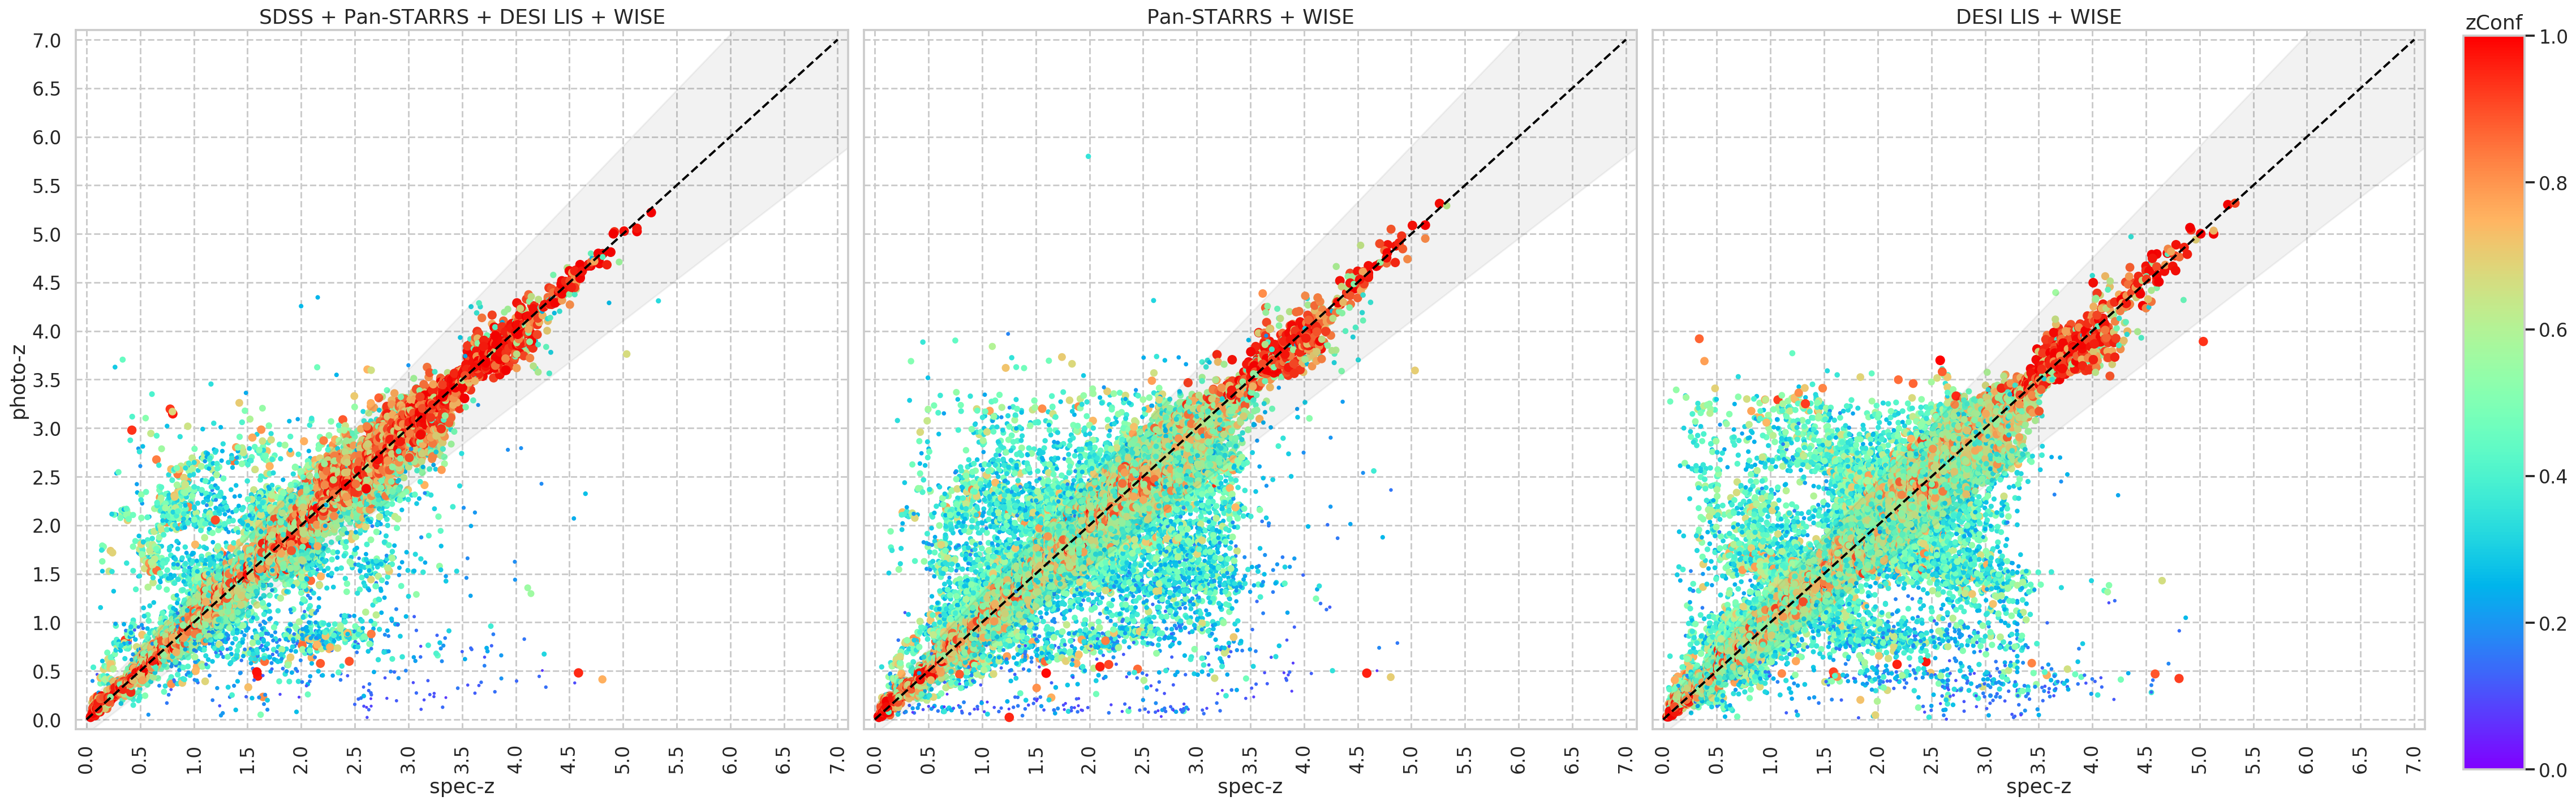
\includegraphics[width=0.9\linewidth]{images/scatterplots-dr16q-wo-train.png}
    \caption{Диаграммы рассеяния прогнозов четырех моделей Photo-z (Pan-STARRS + WISE слева сверху, Pan-STARRS + DESI LIS + WISE справа сверху, DESI LIS + WISE слева снизу и SDSS + PanSTARRS + DESI LIS + WISE справа снизу) на тестовой выборке оптических квазаров SDSS DR16q. По оси абсцисс -- значение spec-z, по оси ординат -- значение прогноза photo-z. Цветом и размером кружка показана мера достоверности прогноза zConf.}
    \label{fig:dr16q_wo_train}
\end{figure*}

Это подтверждается графиками зависимости метрик от целевой переменной (спектральное красное смещение, см. рис. \ref{fig:metrics_spec-z}). Из графиков так же видно, что модель DESI LIS + WISE имеет точность примерно в два раза ниже остальных моделей. Интересно, точность моделей не имеет простой (например, монотонной), зависимости от красного смещения. На разных интервалах красного смещения точность может меняться как одновременно у всех моделей, так и только у некоторых моделей. Вот некоторые наблюдения, сделанные из графиков:
\begin{itemize}
    \item модель DESI LIS + WISE показывает точность существенно хуже модели Pan-STARRS + WISE на $spec-z < 1$, что позволяет сделать предположение о важности фильтров $i$ и $y$ (которые присутствуют в Pan-STARRS, но отсутствуют в DESI LIS) при прогнозе для таких объектов
    \item модель SDSS + Pan-STARRS + DESI LIS + WISE показывает точность существенно выше для области $2.5 < spec-z < 3.5$, что показывает важность фильтра $u$ (который присутствует из используемых обзоров только в SDSS) для прогноза для объектов из этой области.
\end{itemize}

\begin{figure*}[ht]
    \centering
    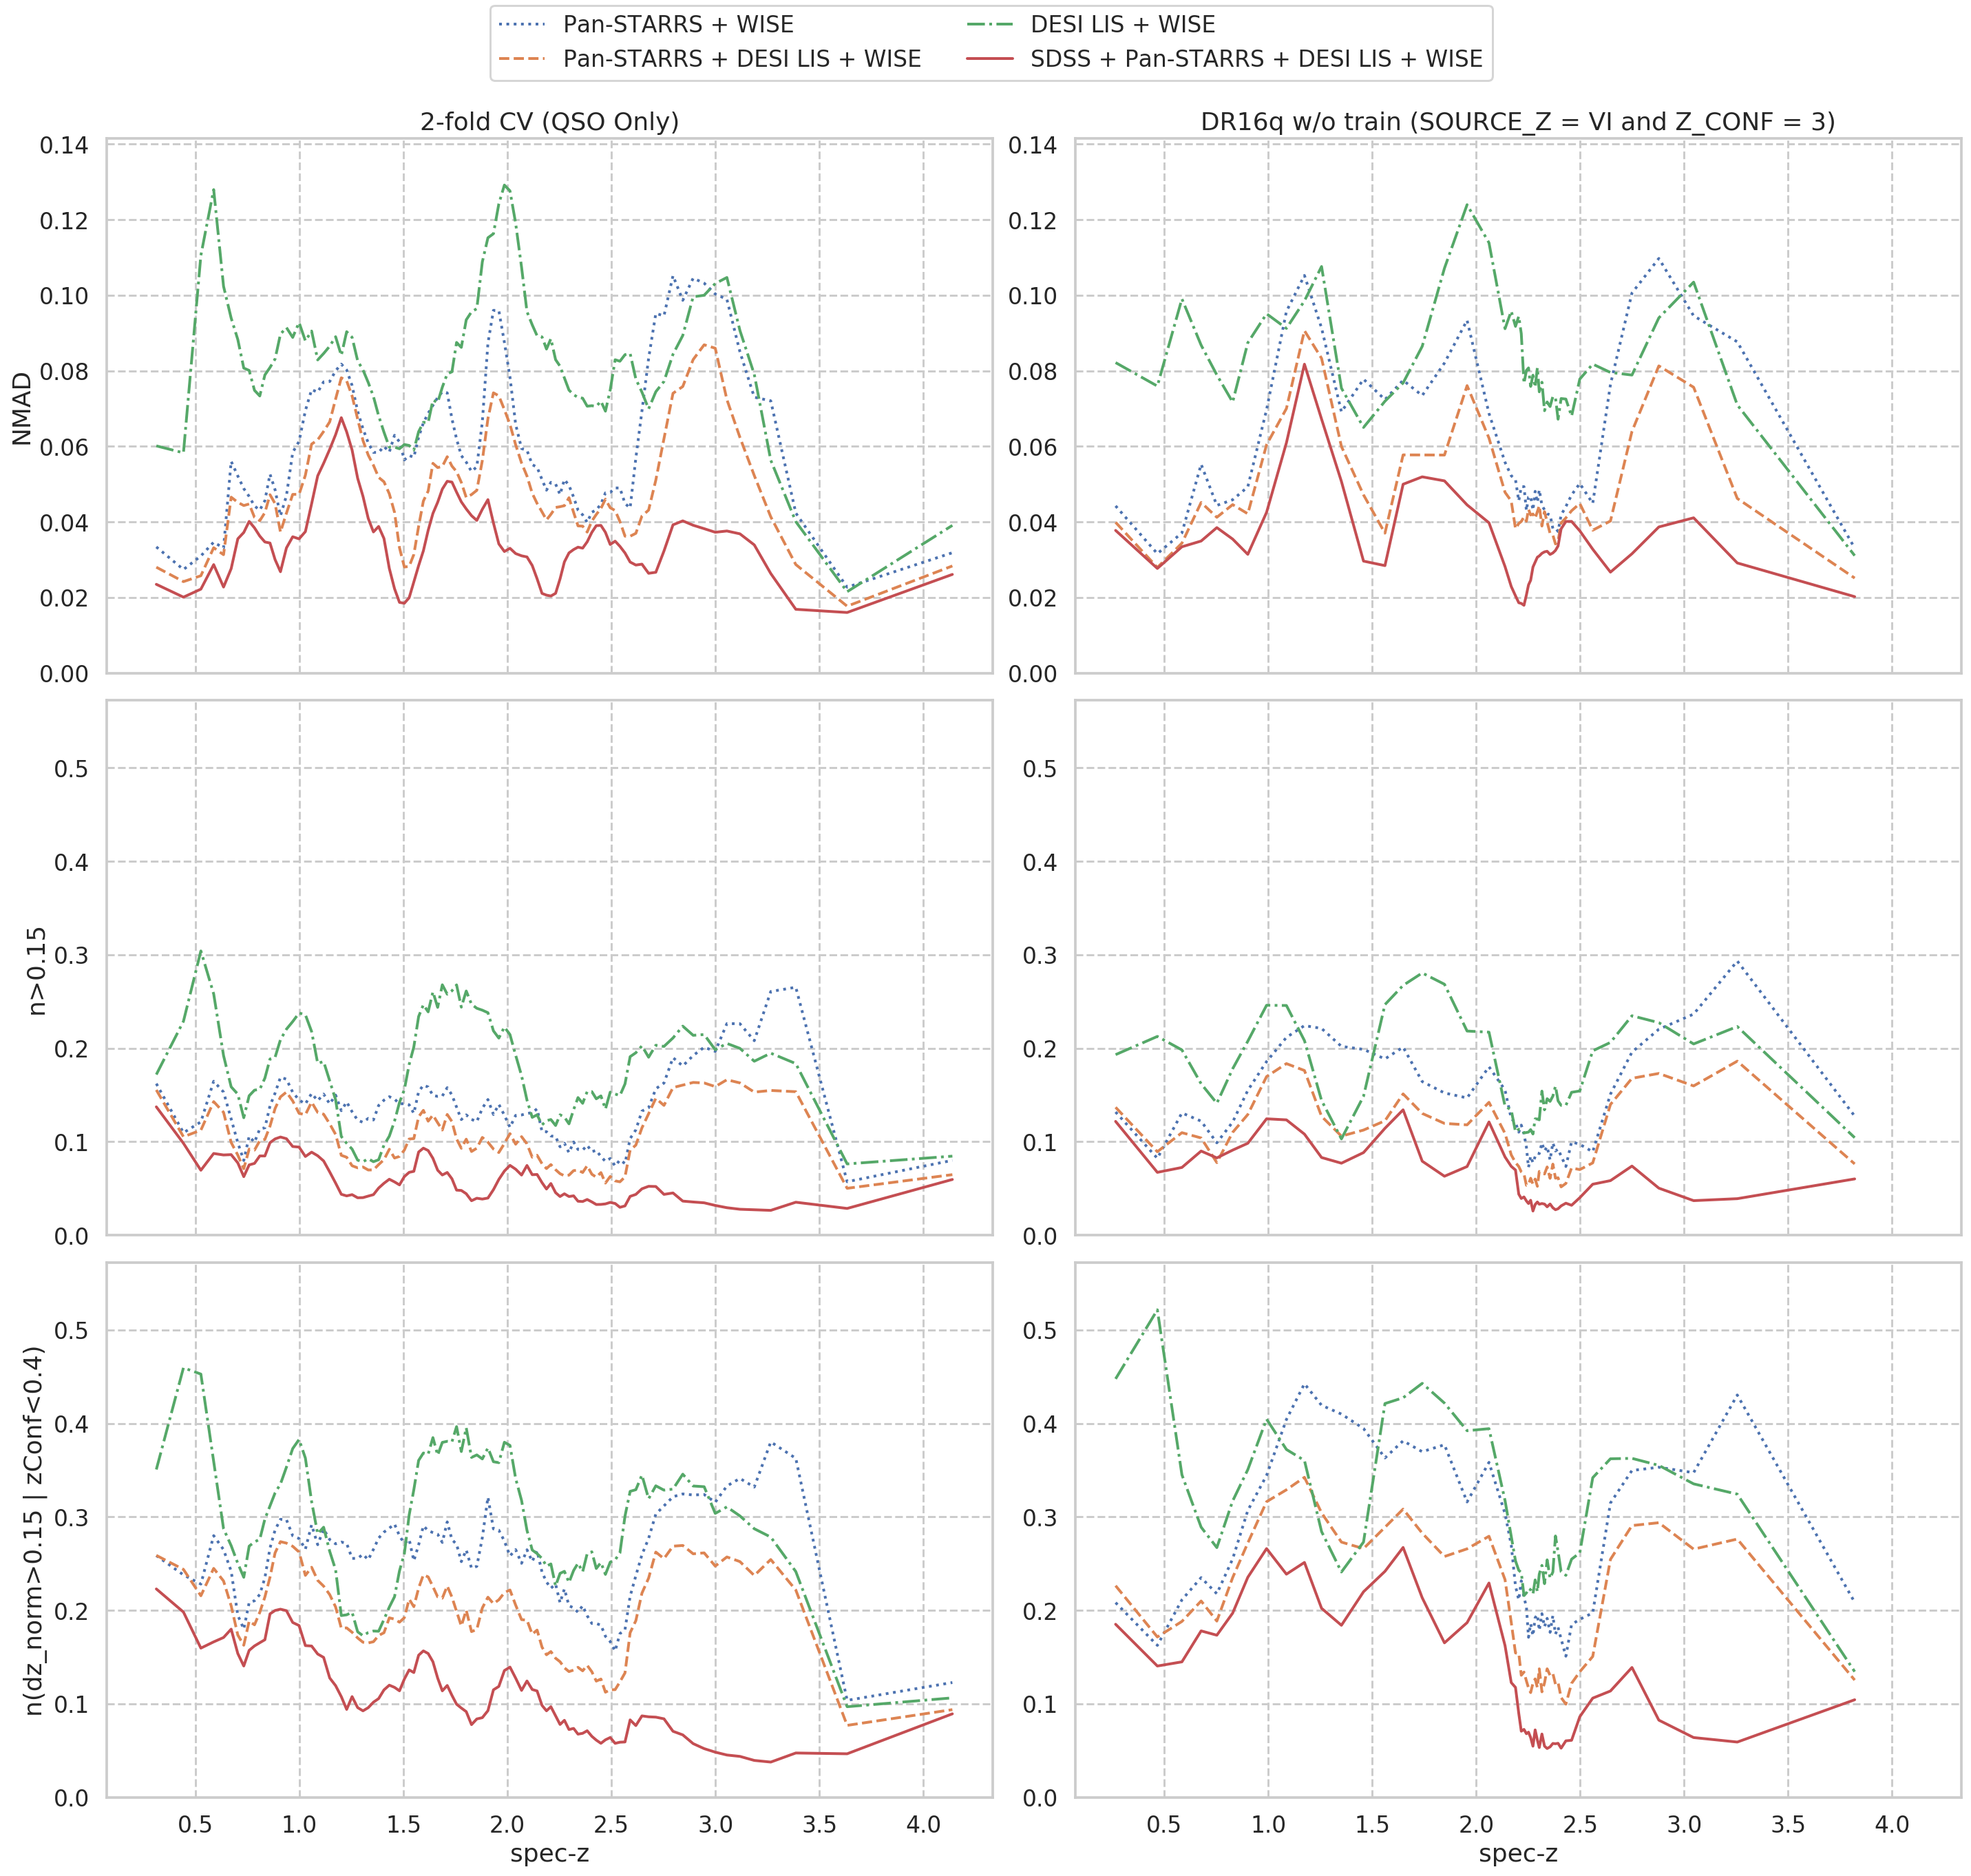
\includegraphics[width=0.9\linewidth]{images/metrics_spec-z.png}
    \caption{Графики метрик точности моделей в зависимости от значения spec-z. На верхних графиках показана метрика $NMAD$ \eqref{eq:nmad}, на нижних графиках -- доля катастрофических выбросов $n_{>0.15}$ \eqref{eq:n015}. Слева -- метрики на двукратной кросс-валидации, справа -- на тестовой выборке оптических квазаров. Модели: Pan-STARRS + WISE -- синий пунктир, DESI LIS + WISE -- зеленый штрих-пунктир, Pan-STARRS + DESI LIS + WISE -- оранжевый штрих, SDSS + DESI LIS + WISE -- красная сплошная кривая.}
    \label{fig:metrics_spec-z}
\end{figure*}

Кроме того была обнаружена зависимость между яркостью объектов и точностью моделей. Мы приводим график только в зависимости от величины $z$ (см. рис. \ref{fig:metrics_z_mag}), однако аналогичные выводы верны, если рассматривать зависимость точности от других величин. Вот некоторые выводы, которые можно сделать:
\begin{itemize}
    \item точность моделей падает на слабых объектов (например, у модели Pan-STARRS до 2.5 раз).
    \item отсутствие фильтров $i$ и $y$ приводит к понижению точности прогнозов для ярких объектов (см. модели DESI LIS + WISE и Pan-STARRS + WISE).
\end{itemize}

\begin{figure*}[ht]
    \centering
    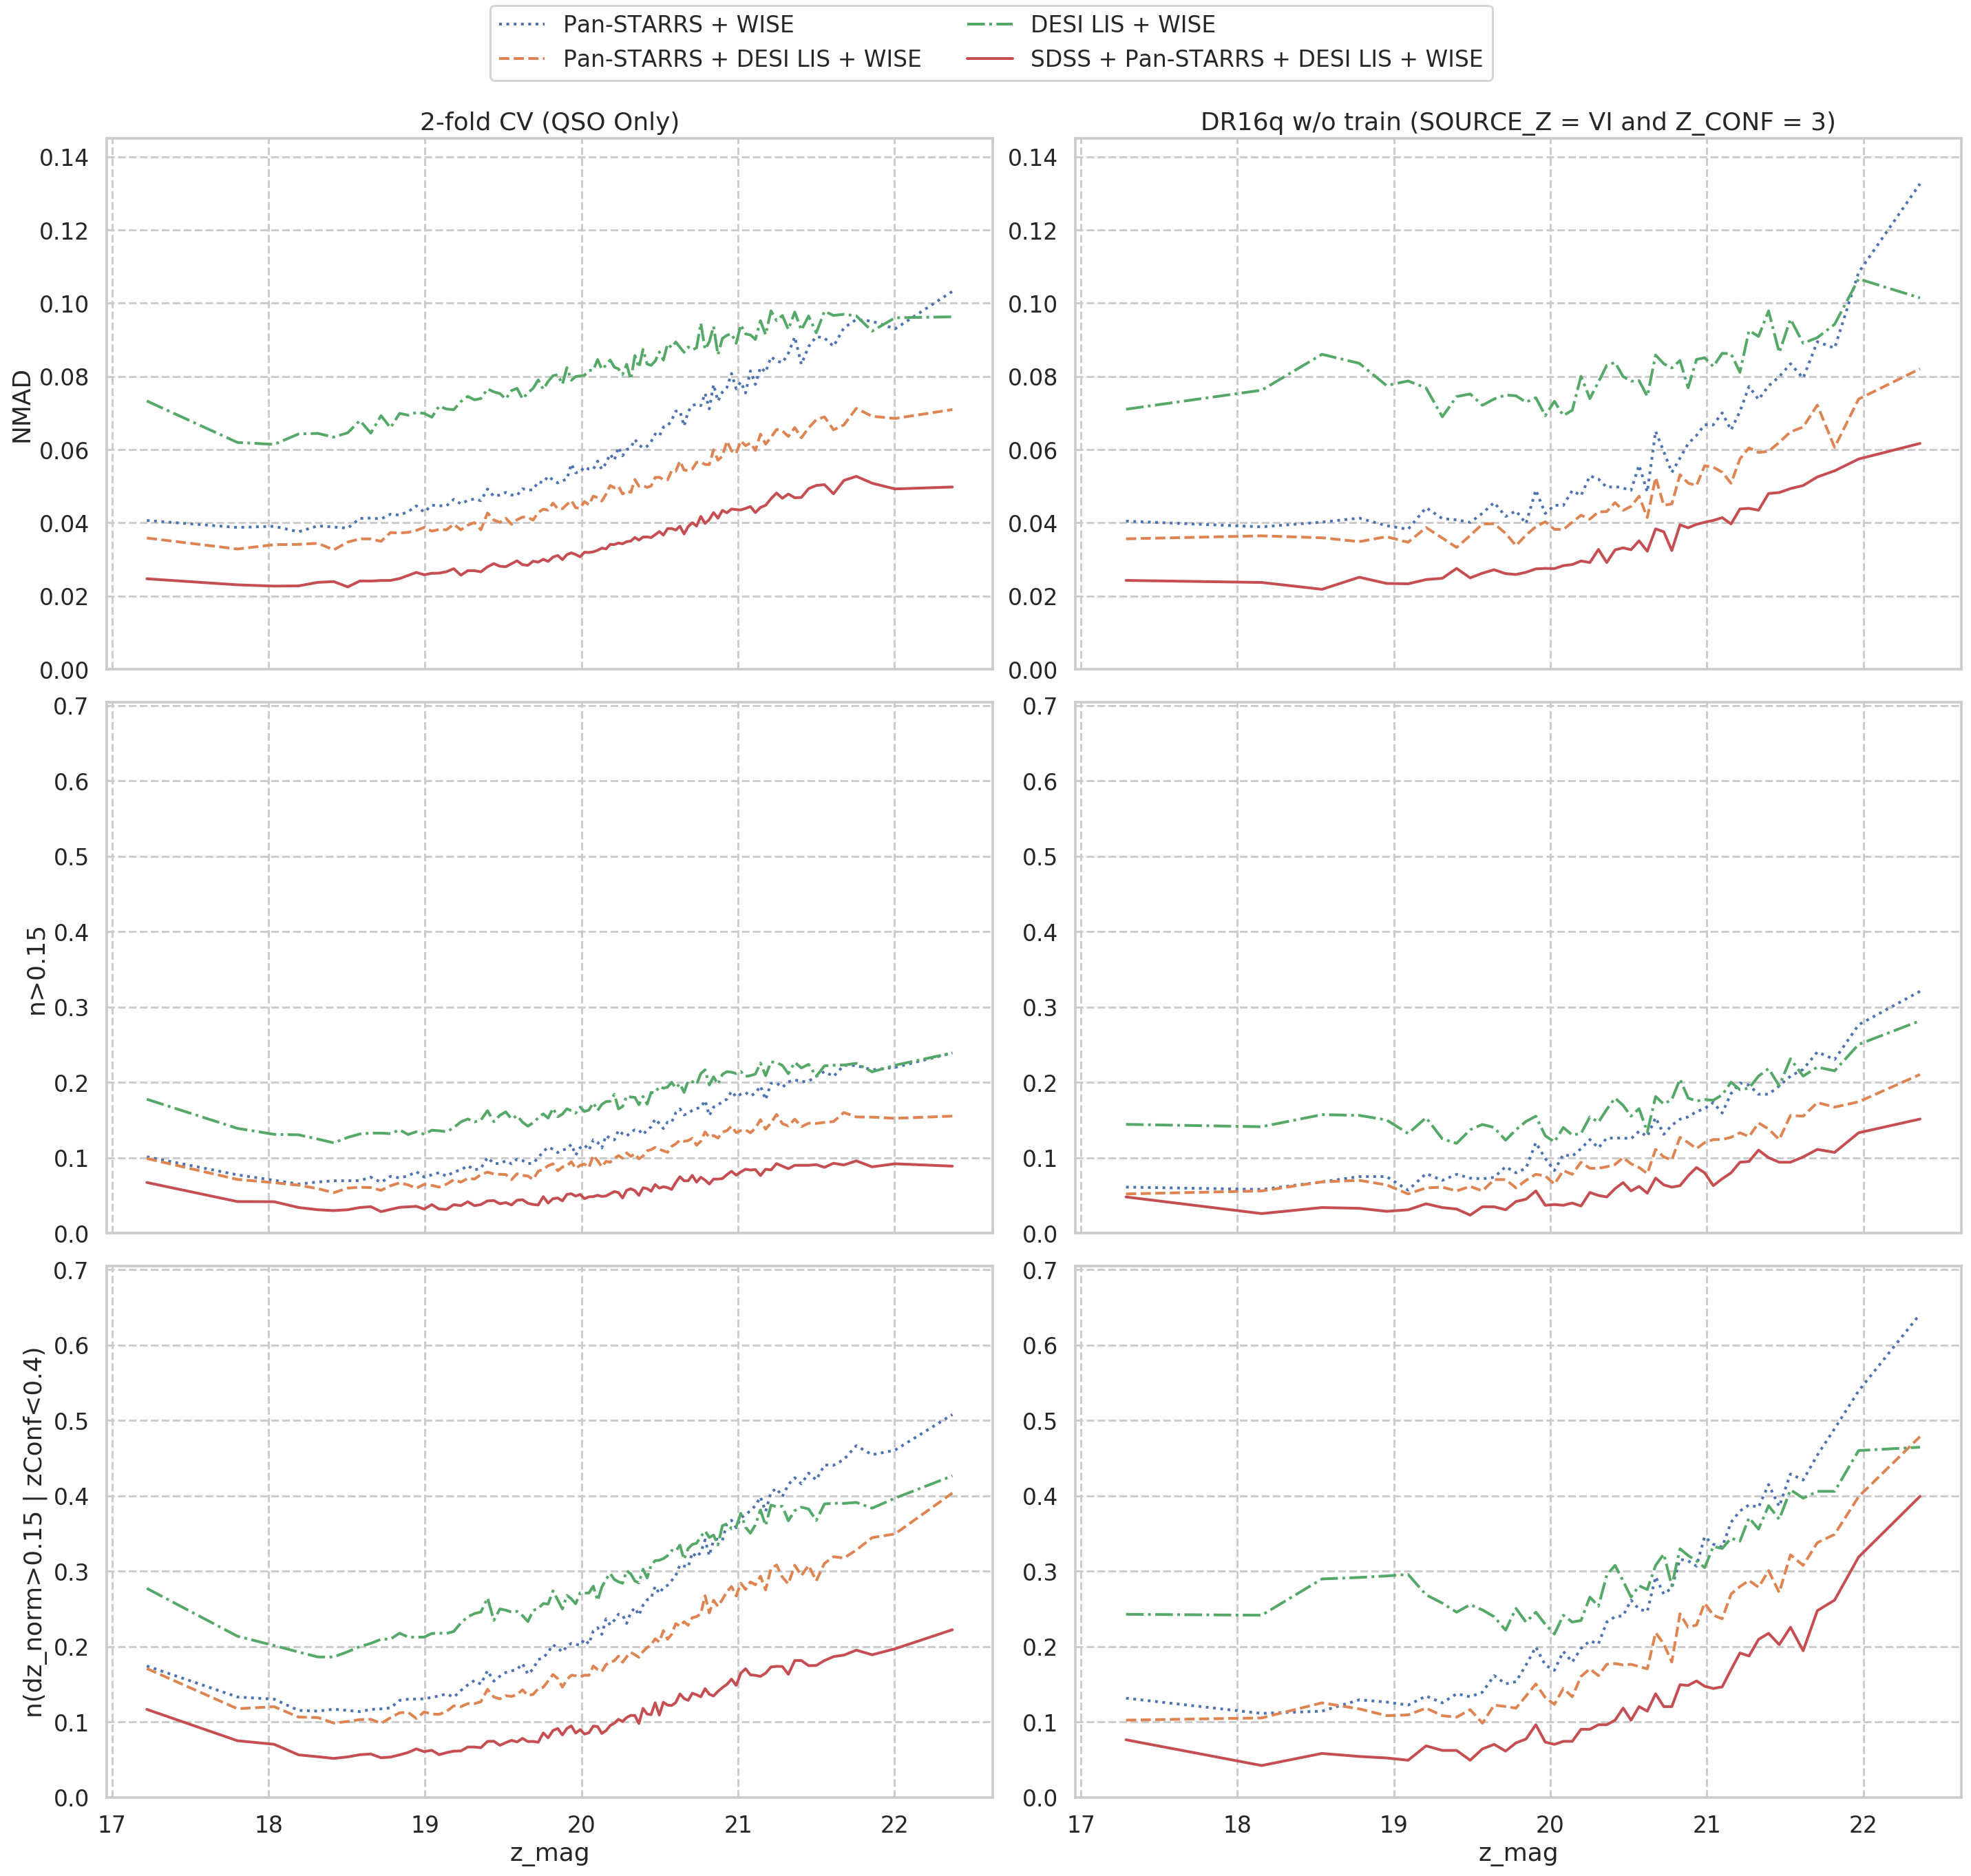
\includegraphics[width=0.9\linewidth]{images/metrics_z-mag.png}
    \caption{Графики метрик точности моделей в зависимости от значения величины z, посчитанной из потоков каталога DESI LIS по формуле гиперболического синуса \eqref{eq:asinhmag}. На верхних графиках показана метрика $NMAD$ \eqref{eq:nmad}, на нижних графиках -- доля катастрофических выбросов $n_{>0.15}$ \eqref{eq:n015}. Слева -- метрики на двукратной кросс-валидации, справа -- на тестовой выборке оптических квазаров. Модели: Pan-STARRS + WISE -- синий пунктир, DESI LIS + WISE -- зеленый штрих-пунктир, Pan-STARRS + DESI LIS + WISE -- оранжевый штрих, SDSS + DESI LIS + WISE -- красная сплошная кривая.}
    \label{fig:metrics_z_mag}
\end{figure*}

\subsection{Stripe82X results}\label{subsec:s82x_results}

В данном разделе приведено описание результатов, полученных на выборке Stripe82X и сравнение с моделями (Ananna, Brescia \ref{}). В целом выводы о поведении моделей повторяют изложенное ранее в пункте \ref{}, поэтому здесь мы заострим внимание на сравнении с моделями других исследователей.

На рис. \ref{fig:s82x} показаны диаграммы рассеяния прогнозов для шести моделей. Можно видеть, что модель на основе четырех широких обзоров SDSS + Pan-STARRS + DESI LIS + WISE так же показвыает себя с лучшей стороны (прогнозы сильнее сгруппрированы вокруг диагонали, меньшая доля выбросов, точные прогнозы имеют бОльшую достоверность). Модель Ananna в свою очередь дает слишком высокую уверенность прогнозов: существенная доля катастрофических выбросов имеет $PDZbest \sim 1$.


\begin{figure*}[ht]
    \centering
    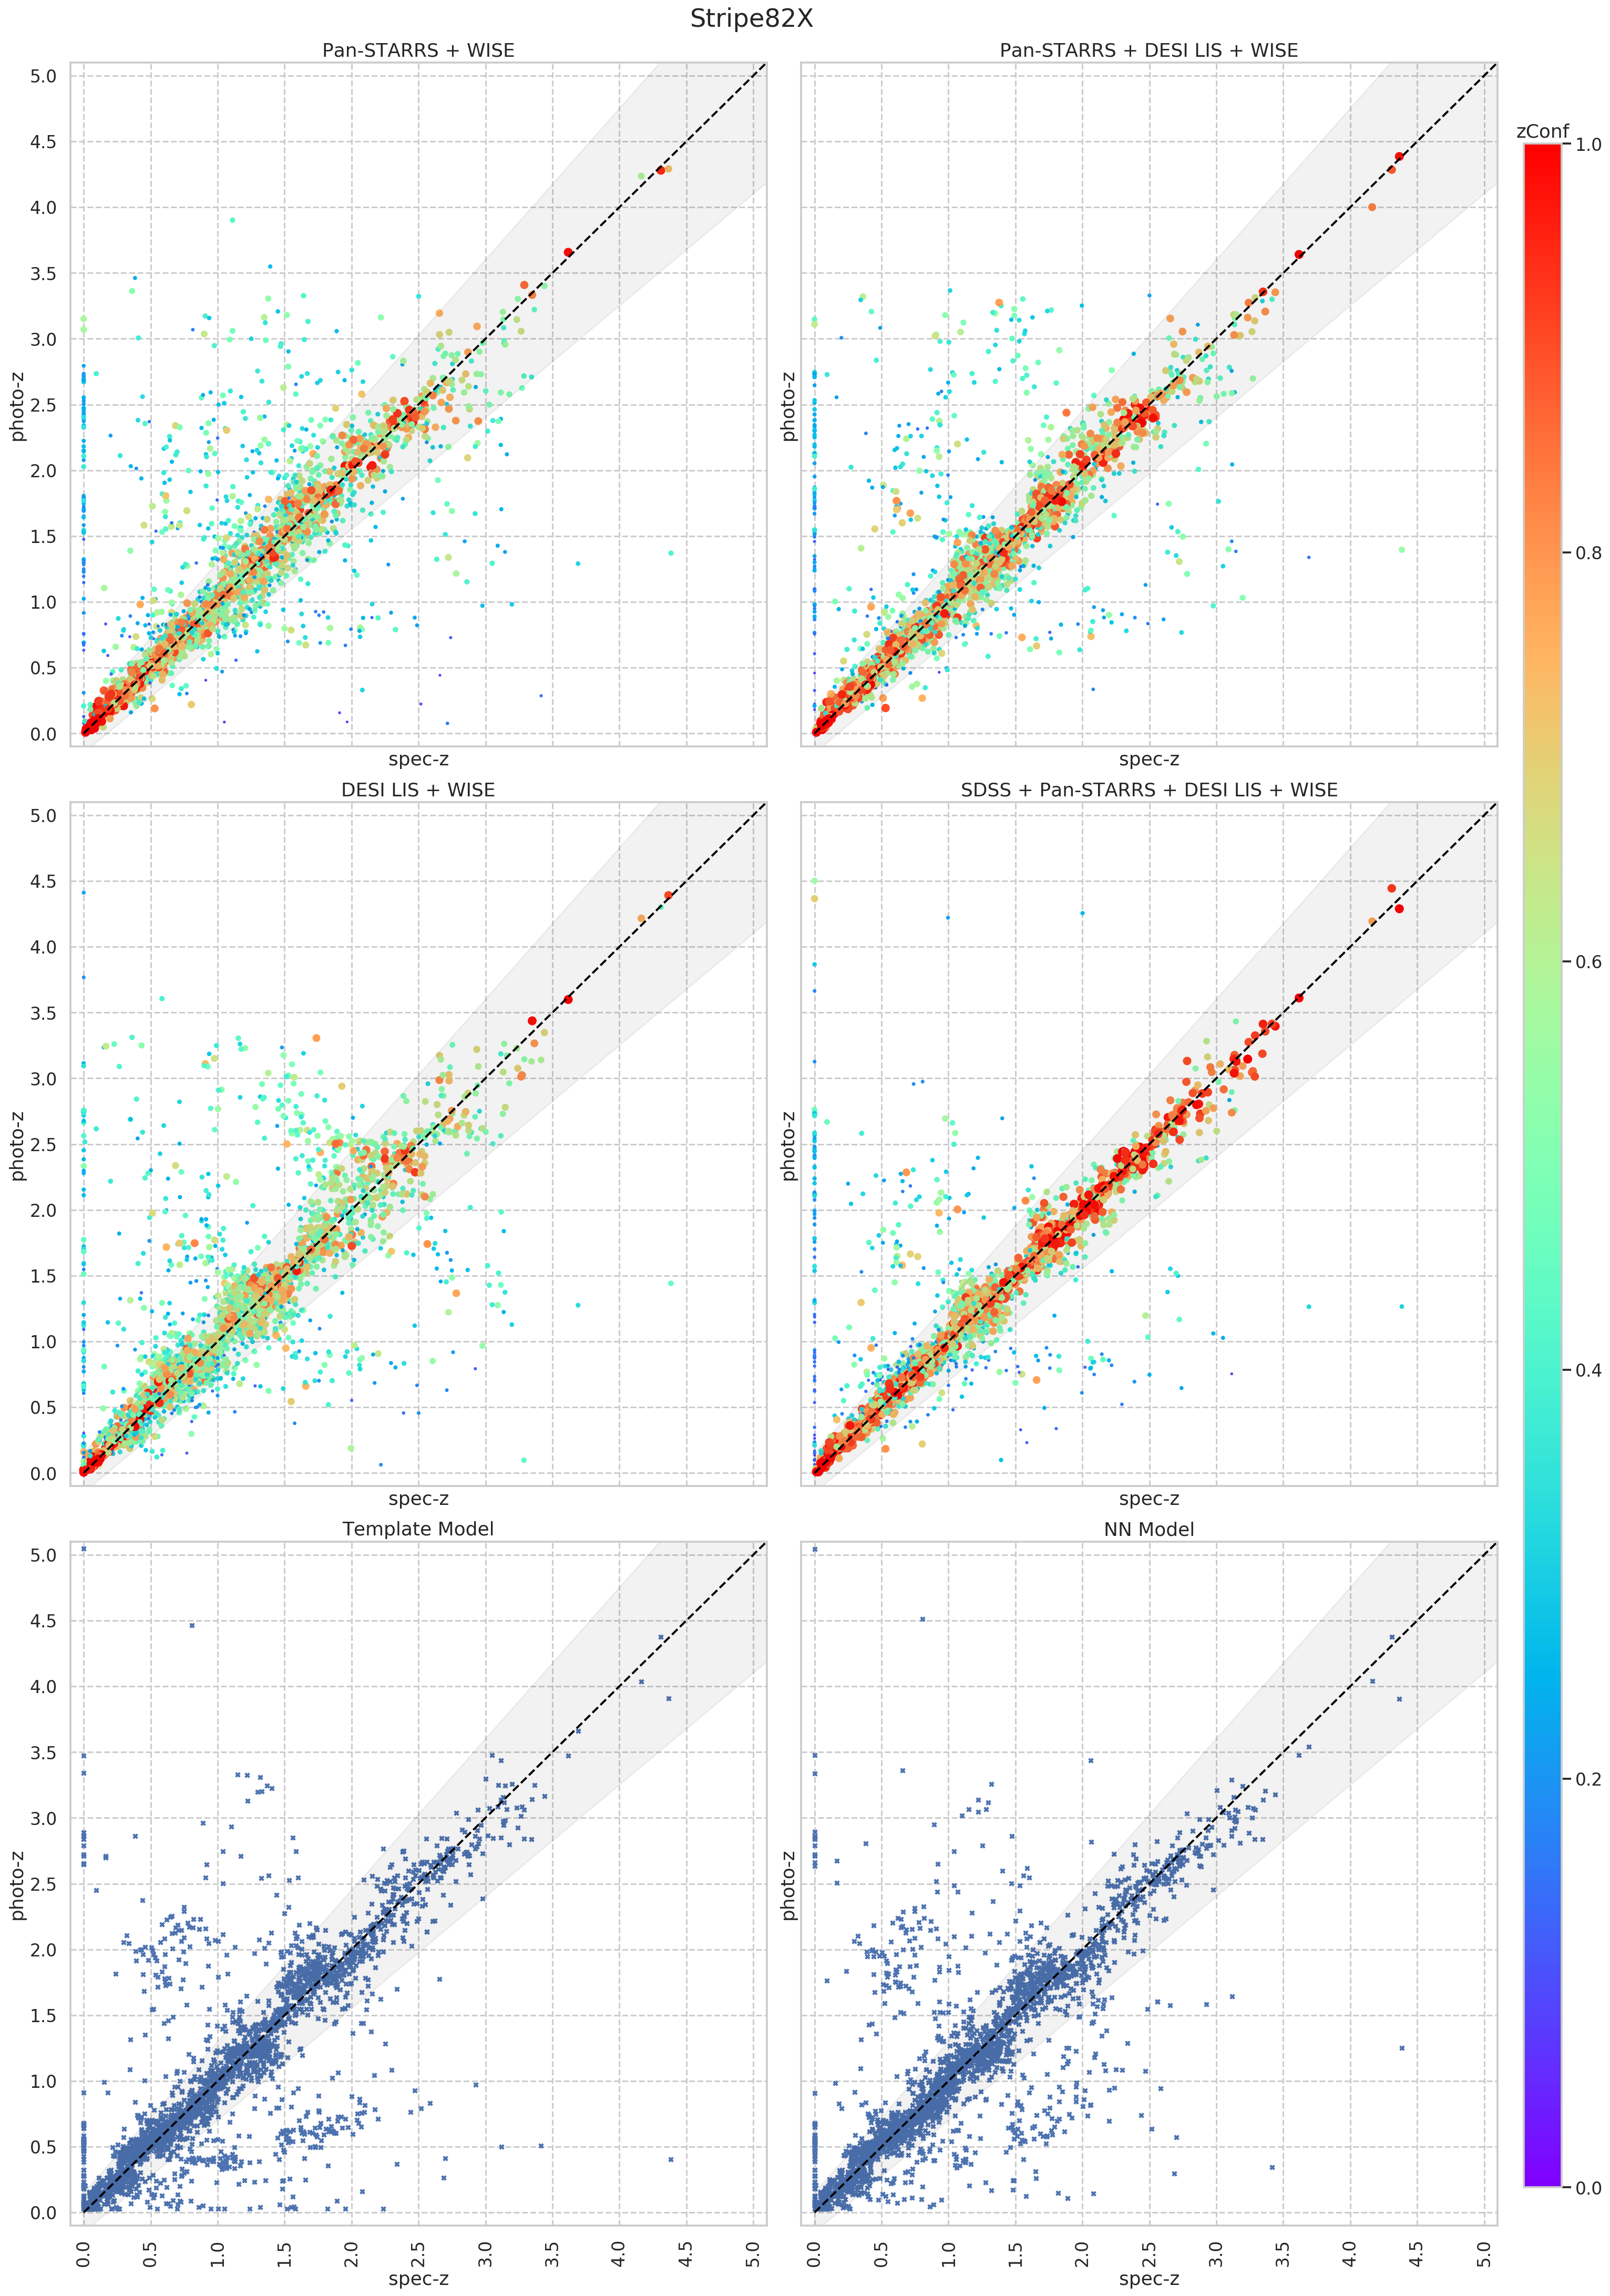
\includegraphics[width=0.9\linewidth]{images/scatterplots-stripe82x.png}
    \caption{Диаграммы рассеяния прогнозов четырех моделей Photo-z (Pan-STARRS + WISE слева сверху, Pan-STARRS + DESI LIS + WISE справа сверху, DESI LIS + WISE слева посередине и SDSS + PanSTARRS + DESI LIS + WISE справа посередине, шаблонная модель (Ananna, 2017) слева снизу и нейросетевая модель (Brescia, 2019) справа снизу) на тестовой выборке рентгеновских объектов Stripe82X. По оси абсцисс -- значение spec-z, по оси ординат -- значение прогноза photo-z. Цветом и размером кружка показана мера достоверности прогноза zConf (PDZbest для Ananna).}
    \label{fig:s82x}
\end{figure*}

\begin{table*}
	\begin{tabular}{llllllllll}
            \hline
            {} & \multicolumn{3}{l}{$All$ (2403 objects)} & \multicolumn{3}{l}{$z_{spec} < 0.5$ (570 objects)} & \multicolumn{3}{l}{$0.5 \leq z_{spec} < 1$ (635 objects)} \\
            {} &               $NMAD$ &        $n>0.15$ &  $C_{68} - 0.68$ &                         $NMAD$ &        $n>0.15$ & $C_{68} - 0.68$ &                                $NMAD$ &        $n>0.15$ &  $C_{68} - 0.68$ \\
            Model          &                      &                 &                  &                                &                 &                 &                                       &                 &                  \\
            \hline
            PW             &                0.057 &           0.149 &            0.042 &                          0.037 &           0.091 &  \textbf{0.022} &                                 0.054 &           0.145 &             0.06 \\
            PDW            &                0.046 &           0.112 &            0.076 &                          0.031 &           0.086 &           0.041 &                                 0.046 &           0.134 &            0.073 \\
            DW             &                0.073 &           0.177 &  \textbf{-0.008} &                          0.047 &           0.112 &           0.032 &                                 0.084 &           0.206 &  \textbf{-0.025} \\
            SPDW           &       \textbf{0.034} &  \textbf{0.089} &            0.104 &                  \textbf{0.03} &  \textbf{0.084} &           0.062 &                        \textbf{0.038} &  \textbf{0.106} &            0.122 \\
            Template Model &                0.066 &           0.177 &           -0.342 &                          0.075 &           0.114 &          -0.499 &                                 0.062 &           0.217 &           -0.289 \\
            NN Model       &                0.066 &            0.16 &           -0.258 &                          0.073 &           0.116 &          -0.396 &                                 0.065 &           0.203 &           -0.193 \\
            \hline
            \end{tabular}
            \caption{Точность моделей в зависимости от красного смещения (spec-z) на выборке Stripe82X для моделей Pan-STARRS + WISE (PW), Pan-STARRS + DESI LIS + WISE (PDW), DESI LIS + WISE (DW), SDSS + Pan-STARRS + DESI LIS + WISE (SPDW), шаблонной модели Ananna \ref{} (Template Model) и нейросетевой модели Brescia \ref{} (NN Model). Для каждого интервала даны метрики $NMAD$ \eqref{eq:nmad}, доля катастрофических выбросов $n_{.0.15}$ \eqref{eq:n015} и калибровка 68-процентных доверительных интервалов $C_{68} - 0.68$ \eqref{eq:c68}.}
\end{table*}

\begin{table*}
	\begin{tabular}{llllllllll}
            \hline
            {} & \multicolumn{3}{l}{$1 \leq z_{spec} < 1.5$ (514 objects)} & \multicolumn{3}{l}{$1.5 \leq z_{spec} < 2$ (369 objects)} & \multicolumn{3}{l}{$2 \leq z_{spec}$ (315 objects)} \\
            {} &                                $NMAD$ &        $n>0.15$ & $C_{68} - 0.68$ &                                $NMAD$ &        $n>0.15$ &  $C_{68} - 0.68$ &                          $NMAD$ &        $n>0.15$ &  $C_{68} - 0.68$ \\
            Model          &                                       &                 &                 &                                       &                 &                  &                                 &                 &                  \\
            \hline
            PW             &                                 0.081 &           0.187 &           0.034 &                                 0.082 &           0.163 &            0.057 &                           0.057 &           0.184 &            0.037 \\
            PDW            &                                 0.061 &           0.105 &           0.073 &                                 0.042 &           0.103 &            0.128 &                           0.046 &           0.133 &            0.088 \\
            DW             &                                 0.083 &            0.14 &  \textbf{0.001} &                                 0.076 &           0.255 &  \textbf{-0.032} &                           0.088 &           0.203 &  \textbf{-0.032} \\
            SPDW           &                        \textbf{0.048} &  \textbf{0.088} &           0.122 &                        \textbf{0.031} &  \textbf{0.065} &            0.144 &                  \textbf{0.029} &  \textbf{0.098} &            0.072 \\
            Template Model &                                  0.07 &           0.206 &          -0.285 &                                 0.075 &            0.22 &           -0.279 &                           0.045 &           0.111 &           -0.331 \\
            NN Model       &                                 0.069 &           0.167 &          -0.207 &                                 0.067 &           0.182 &           -0.192 &                           0.047 &           0.114 &           -0.302 \\
            \hline
            \end{tabular}
            \caption{Точность моделей в зависимости от красного смещения (spec-z) на выборке Stripe82X для моделей Pan-STARRS + WISE (PW), Pan-STARRS + DESI LIS + WISE (PDW), DESI LIS + WISE (DW), SDSS + Pan-STARRS + DESI LIS + WISE (SPDW), шаблонной модели Ananna \ref{} (Template Model) и нейросетевой модели Brescia \ref{} (NN Model). Для каждого интервала даны метрики $NMAD$ \eqref{eq:nmad}, доля катастрофических выбросов $n_{.0.15}$ \eqref{eq:n015} и калибровка 68-процентных доверительных интервалов $C_{68} - 0.68$ \eqref{eq:c68}.}
\end{table*}




\begin{table*}
	\begin{tabular}{llllllllll}
            \hline
            {} & \multicolumn{3}{l}{$z_{mag} < 19$ (522 objects)} & \multicolumn{3}{l}{$19 \leq z_{mag} < 20$ (608 objects)} & \multicolumn{3}{l}{$20 \leq z_{mag} < 20.5$ (403 objects)} \\
            {} &                       $NMAD$ &        $n>0.15$ & $C_{68} - 0.68$ &                               $NMAD$ &        $n>0.15$ & $C_{68} - 0.68$ &                                 $NMAD$ &        $n>0.15$ & $C_{68} - 0.68$ \\
            Model          &                              &                 &                 &                                      &                 &                 &                                        &                 &                 \\
            \hline
            PW             &                        0.034 &           0.046 &           0.035 &                                0.043 &           0.062 &           0.088 &                                  0.064 &           0.119 &           0.035 \\
            PDW            &                        0.027 &            0.04 &           0.044 &                                0.036 &           0.064 &           0.116 &                                  0.046 &           0.102 &           0.107 \\
            DW             &                        0.039 &           0.084 &  \textbf{0.025} &                                0.068 &           0.112 &  \textbf{0.012} &                                  0.076 &           0.156 &  \textbf{0.012} \\
            SPDW           &               \textbf{0.024} &  \textbf{0.029} &           0.081 &                       \textbf{0.028} &  \textbf{0.041} &           0.131 &                         \textbf{0.033} &  \textbf{0.074} &           0.107 \\
            Template Model &                        0.061 &           0.092 &          -0.536 &                                0.062 &           0.145 &          -0.399 &                                  0.064 &           0.166 &           -0.38 \\
            NN Model       &                        0.062 &           0.092 &          -0.464 &                                0.058 &           0.133 &          -0.308 &                                  0.061 &           0.144 &          -0.288 \\
            \hline
            \end{tabular}
            \caption{Точность моделей в зависимости от величины в фильтре $z$, посчитанной по поткам DESI LIS с ипользованием формулы \eqref{eq:asinhmag}, на выборке Stripe82X для моделей Pan-STARRS + WISE (PW), Pan-STARRS + DESI LIS + WISE (PDW), DESI LIS + WISE (DW), SDSS + Pan-STARRS + DESI LIS + WISE (SPDW), шаблонной модели Ananna \ref{} (Template Model) и нейросетевой модели Brescia \ref{} (NN Model). Для каждого интервала даны метрики $NMAD$ \eqref{eq:nmad}, доля катастрофических выбросов $n_{.0.15}$ \eqref{eq:n015} и калибровка 68-процентных доверительных интервалов $C_{68} - 0.68$ \eqref{eq:c68}.}
\end{table*}

\begin{table*}
	\begin{tabular}{lllllll}
            \hline
            {} & \multicolumn{3}{l}{$20.5 \leq z_{mag} < 21$ (358 objects)} & \multicolumn{3}{l}{$21 \leq z_{mag} < 23$ (510 objects)} \\
            {} &                                 $NMAD$ &        $n>0.15$ &  $C_{68} - 0.68$ &                               $NMAD$ &       $n>0.15$ & $C_{68} - 0.68$ \\
            Model          &                                        &                 &                  &                                      &                &                 \\
            \hline
            PW             &                                  0.066 &           0.176 &            0.035 &                                 0.12 &          0.359 &  \textbf{0.008} \\
            PDW            &                                  0.056 &            0.12 &            0.074 &                                0.081 &          0.243 &           0.036 \\
            DW             &                                  0.088 &           0.218 &  \textbf{-0.012} &                                0.119 &          0.337 &           -0.08 \\
            SPDW           &                         \textbf{0.044} &  \textbf{0.106} &            0.105 &                       \textbf{0.063} &  \textbf{0.21} &           0.095 \\
            Template Model &                                  0.057 &           0.201 &           -0.219 &                                0.087 &          0.294 &          -0.135 \\
            NN Model       &                                  0.062 &            0.17 &           -0.135 &                                 0.09 &          0.267 &          -0.055 \\
            \hline
            \end{tabular}
            \caption{Точность моделей в зависимости от величины в фильтре $z$, посчитанной по поткам DESI LIS с ипользованием формулы \eqref{eq:asinhmag}, на выборке Stripe82X для моделей Pan-STARRS + WISE (PW), Pan-STARRS + DESI LIS + WISE (PDW), DESI LIS + WISE (DW), SDSS + Pan-STARRS + DESI LIS + WISE (SPDW), шаблонной модели Ananna \ref{} (Template Model) и нейросетевой модели Brescia \ref{} (NN Model). Для каждого интервала даны метрики $NMAD$ \eqref{eq:nmad}, доля катастрофических выбросов $n_{.0.15}$ \eqref{eq:n015} и калибровка 68-процентных доверительных интервалов $C_{68} - 0.68$ \eqref{eq:c68}.}
\end{table*}




\begin{table*}
	\begin{tabular}{llllllllll}
            \hline
            {} & \multicolumn{3}{l}{$FSoft < 3e-15$ (55 objects)} & \multicolumn{3}{l}{$FSoft < 1e-14$ (983 objects)} & \multicolumn{3}{l}{$FSoft < 4e-14$ (2055 objects)} \\
            {} &                       $NMAD$ &        $n>0.15$ & $C_{68} - 0.68$ &                        $NMAD$ &        $n>0.15$ & $C_{68} - 0.68$ &                         $NMAD$ &        $n>0.15$ &  $C_{68} - 0.68$ \\
            Model          &                              &                 &                 &                               &                 &                 &                                &                 &                  \\
            \hline
            PW             &                        0.056 &           0.182 &           0.029 &                         0.067 &           0.186 &           0.032 &                           0.06 &           0.154 &            0.044 \\
            PDW            &                         0.05 &           0.164 &           0.084 &                          0.05 &           0.133 &            0.08 &                          0.047 &           0.115 &            0.079 \\
            DW             &                        0.059 &             0.2 &  \textbf{0.011} &                         0.075 &           0.202 &  \textbf{0.002} &                          0.074 &           0.179 &  \textbf{-0.007} \\
            SPDW           &               \textbf{0.034} &  \textbf{0.127} &           0.102 &                \textbf{0.038} &  \textbf{0.109} &           0.098 &                 \textbf{0.035} &  \textbf{0.093} &            0.108 \\
            Template Model &                        0.059 &             0.2 &          -0.425 &                         0.061 &           0.165 &           -0.28 &                          0.064 &           0.172 &           -0.323 \\
            NN Model       &                        0.074 &  \textbf{0.127} &          -0.244 &                         0.064 &           0.149 &          -0.199 &                          0.065 &           0.155 &           -0.243 \\
            \hline
            \end{tabular}
            \caption{Точность моделей в зависимости рентгеновского потока $FSoft$ на выборке Stripe82X для моделей Pan-STARRS + WISE (PW), Pan-STARRS + DESI LIS + WISE (PDW), DESI LIS + WISE (DW), SDSS + Pan-STARRS + DESI LIS + WISE (SPDW), шаблонной модели Ananna \ref{} (Template Model) и нейросетевой модели Brescia \ref{} (NN Model). Интервалы по рентгеновскому потоку соответствуют глубине (сколько летнего) обзора eRosita. Для каждого интервала даны метрики $NMAD$ \eqref{eq:nmad}, доля катастрофических выбросов $n_{.0.15}$ \eqref{eq:n015} и калибровка 68-процентных доверительных интервалов $C_{68} - 0.68$ \eqref{eq:c68}.}
\end{table*}

\subsection{PDZ reliability}

\begin{figure*}[ht]
    \centering
    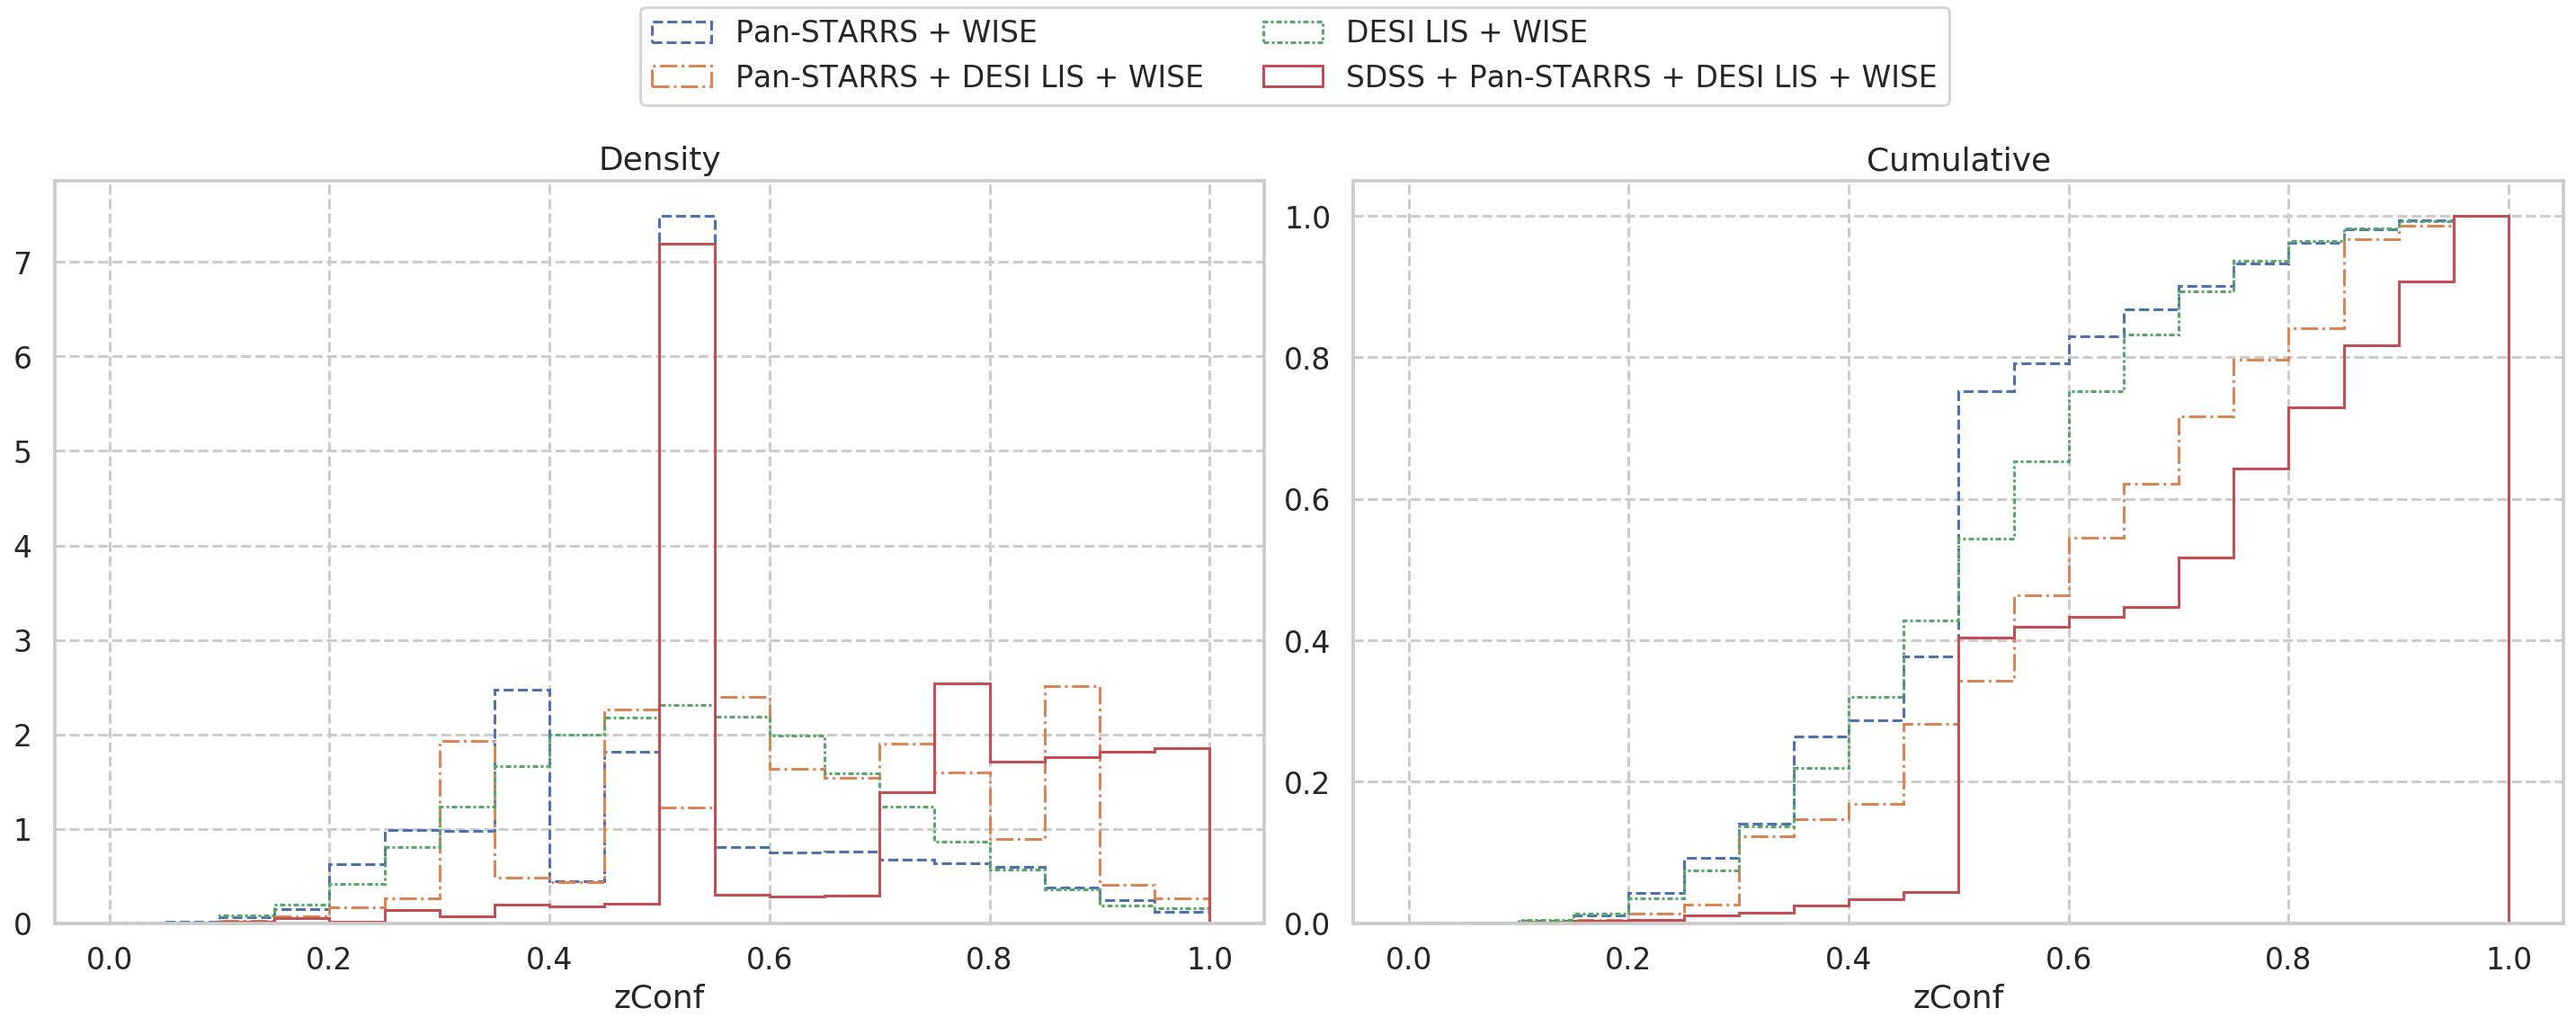
\includegraphics[width=0.9\linewidth]{images/zconf-cal-dr16q.png}
    \caption{zConf distribution on DR16q test sample}
    \label{fig:zconf-cal-dr16q}
\end{figure*}

\begin{figure*}[ht]
    \centering
    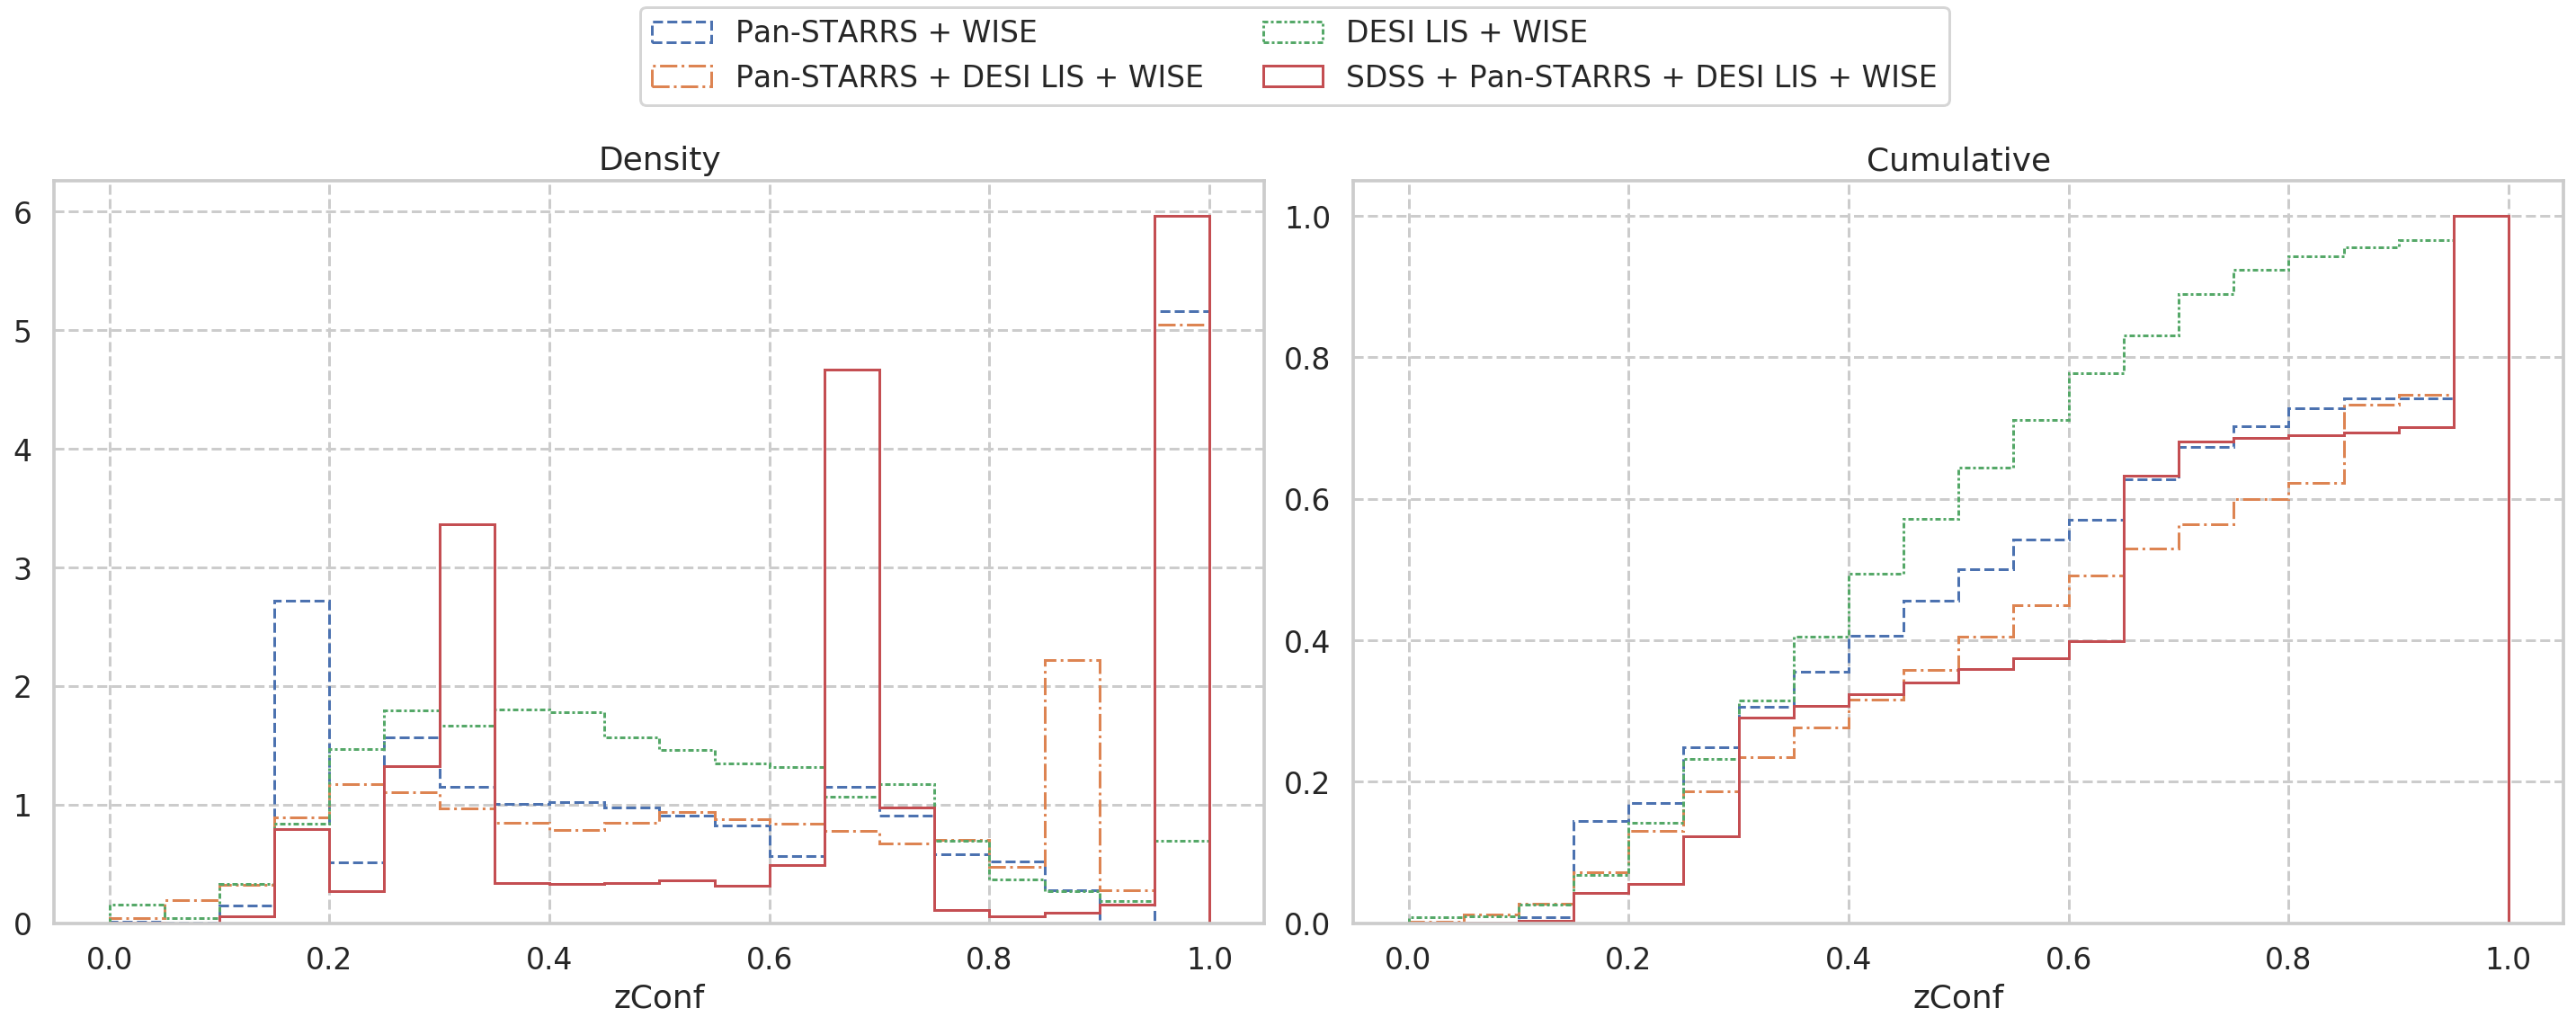
\includegraphics[width=0.9\linewidth]{images/zconf-cal-stripe82X.png}
    \caption{zConf distribution on Stripe82X test sample}
    \label{fig:zconf-cal-stripe82X}
\end{figure*}

% ===============================================================================
% ===============================================================================
% ===============================================================================

\section{Conclusion}

% В рамках работы было построено множество моделей photo-z на основе различных признаков, которые строятся по данным трех современных фотометрических обзоров~--- SDSS, Pan-STARRS1 и DESI Legacy Imaging Survey. Обучающая выборка состоит из $\sim$580000 оптических квазаров и галактик и сбалансирована, чтобы аппроксимировать распределение рентгеновских объектов. Разметка взята из спектрального каталога оптических объектов SDSS.

% На тестовой выборке рентгеновских объектов поля Stripe82X \cite{bib:ananna}, за счет использования данных всех трех вышеупомянутых обзоров, была достигнута точность по метрикам $NMAD$ и доля выбросов $n_{>0.15}$ значительно выше (почти в 2 раза), чем точность лучших моделей известных в литературе (SOTA), что является основным результатом работы. Для лучшей модели / шаблонной модели \cite{bib:ananna} / нейросетевой модели \cite{bib:brescia} на выборке Stripe82X получены значения метрик $NMAD$ = 0.034 / 0.065 / 0.066 и $n_{>0.15}$ = 0.088 / 0.170 / 0.156, соответственно.

The proposed photo-z models based on Random Forests show accuracy (up to 2 times) better than current SOTA results in the literature (on Stripe82X field). The main accuracy improvement comes from using a large training sample ($\sim$600k objects) with features from modern wide photometric surveys. First optical spectroscopic observations of eRosita sources show that the proposed photo-z models are effective in the ongoing search for distant X-ray quasars (see e.g. \citep{2020MNRAS.497.1842M,2020AstL...46..149K,2020AstL...46..429D}).

The presented photo-z models are integrated into the SRGz system designed to construct a three-dimensional map of X-ray sources on the Eastern Galactic Hemisphere of the SRG/eRosita All-Sky survey. The SRGz system is developed in the science working group of RU eROSITA consortium on X-ray source detection, identification, and eROSITA source catalog in the High Energy Astrophysics Department at Space Research Institute of the Russian Academy of Sciences.

% ===============================================================================
% ===============================================================================
% ===============================================================================

\section{Discussion}

Провалы в точности по zspec. Переход на ансамбли нейронных сетей. Источник данных о поглощении на всем небе?

\section*{Acknowledgments}
..

% bibliograpgy 
\bibliographystyle{mnras}
\bibliography{main}

\appendix

\section{..}

\end{document}
